\documentclass[11pt]{beamer}
\usetheme{JuanLesPins}
\usepackage[utf8]{inputenc}
\usepackage[spanish]{babel}
\usepackage{amsmath}
\usepackage{amsfonts}
\usepackage{amssymb}
\usepackage{graphicx}
\usepackage{adjustbox}
\usepackage{array}
\spanishdecimal{.}
\author{M. en E. Sergio Nava}
\title{Variables Aleatorias Contínuas}
%\setbeamercovered{transparent} 
%\setbeamertemplate{navigation symbols}{} 
%\logo{} 
%\institute{} 
\date{Viernes 12 de octubre de 2018} 
%\subject{} 

\AtBeginSection[]  % The commands within the following {} will be executed at the start of each section.
{
\begin{frame} % Within each "frame" there will be one or more "slides."  
\frametitle{Presentation Outline} % This is the title of the outline.
\tableofcontents[currentsection]  % This will display the table of contents and highlight the current section.
\end{frame}
} % Do not include the preceding set of commands if you prefer not to have a recurring outline displayed during your presentation.


\begin{document}

\begin{frame}
\titlepage
\end{frame}


%\begin{frame}
%\tableofcontents
%\end{frame}



\section{Distribución de probabilidad de Variables Aleatorias Contínuas}
\begin{frame}{Distribuci\'on de probabilidad de v.a. continuas}

Hay dos diferencias principales entre el manejo de v.a. continuas con su contraparte discreta.
\begin{enumerate}
\item Ya no se habla de la probabilidad de que una variable aleatoria tome un determinado valor. En su lugar se habla de la probabilidad de que la v. a. asuma un valor dentro de cierto intervalo dado.

\item La probabilidad de que la v.a. tome un valor dentro de un determinado intervalo dado de ${ x }_{ 1 }$ a ${ x }_{ 2 }$ se define como el área bajo la gráfica de la función de densidad de probabilidad entre ${ x }_{ 1 }$ y ${ x }_{ 2 }$. 
\end{enumerate}
{\tiny Esto implica que la probabilidad de que la v.a. continua asuma exactamente determinado valor es cero, porque el área bajo la gráfica de $f(x)$ en un solo punto es cero.}

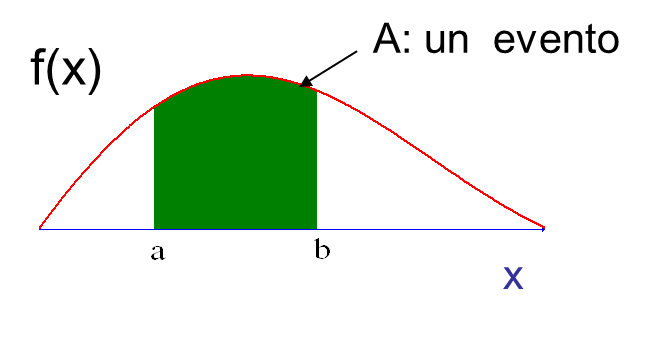
\includegraphics[scale=.4]{ilustraciones/12.png} 
%ilustracion12%
\end{frame}

\begin{frame}{Distribuci\'on de probabilidad de v.a. continuas}
Se llamar\'a a $f(x)$ la \textbf{función de densidad de probabilidad} de una variable aleatoria $X$, si satisface que: 
\begin{enumerate}
	\item$$f\left( x \right) \ge 0,\quad x\in \Re $$

	\item$$\int _{ -\infty  }^{ \infty  }{ f\left( x \right) dx } =1$$

	\item$$P({ x }_{ 1 }\le X\le { x }_{ 2 })=\int _{ { x }_{ 1 } }^{ { x }_{ 2 } }{ f\left( y \right)  } dy$$
\end{enumerate}
\end{frame}

\begin{frame}{Funci\'on de Distribuci\'on Acumulada}

Una funci\'on $F(x)$ es una función de distribuci\'on si y sólo si cumplen las siguientes condiciones:
\begin{enumerate}
	\item $\lim _{ x\rightarrow -\infty  }{ \quad F\left( x \right)  } =0 \mbox{  y  }\lim _{ x\rightarrow +\infty  }{ \quad F\left( x \right)  } =1$.
	\bigskip
	\item $F(x)$ es una funci\'on no decreciente.
	\bigskip	
	\item $F(x)$ es continua por la derecha:
	$\forall h>0,\quad \lim _{ h\rightarrow 0 }{ \quad F(x+h)=F(X) }$ 

\end{enumerate}

\end{frame}

\begin{frame}{Funci\'on de Distribuci\'on Acumulada de v.a. Continuas}
La \textbf{función de distribución acumulada} de la variable aleatoria $X$ es la probabilidad de que $X$ sea menor o igual a un valor específico $x$, esta dada por:

$$F(X)\equiv P(X\le x)=\int _{ -\infty  }^{ x }{ f(y) } dy$$

por lo tanto

$$P(a\le X\le b)=\int _{ a }^{ b }{ f(y) } dy=F(b)-F(a)$$
\end{frame}

\begin{frame}{Funci\'on de Distribuci\'on Acumulada de v.a. Continuas}
$$P(a\le X\le b)=\int _{ a }^{ b }{ f(y) } dy=F(b)-F(a)$$
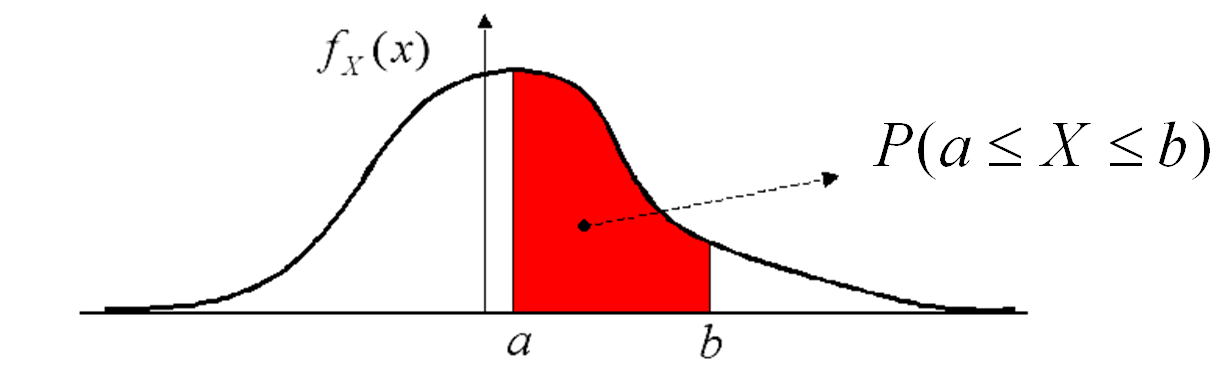
\includegraphics[scale=0.5]{ilustraciones/13.png} 
%ilustracion13%
\end{frame}

\begin{frame}{Funci\'on de Distribuci\'on Acumulada de v.a. Continuas}
Una variable aleatoria  X es continua si su funci\'on de distribuci\'on $F(x)$ es continua.
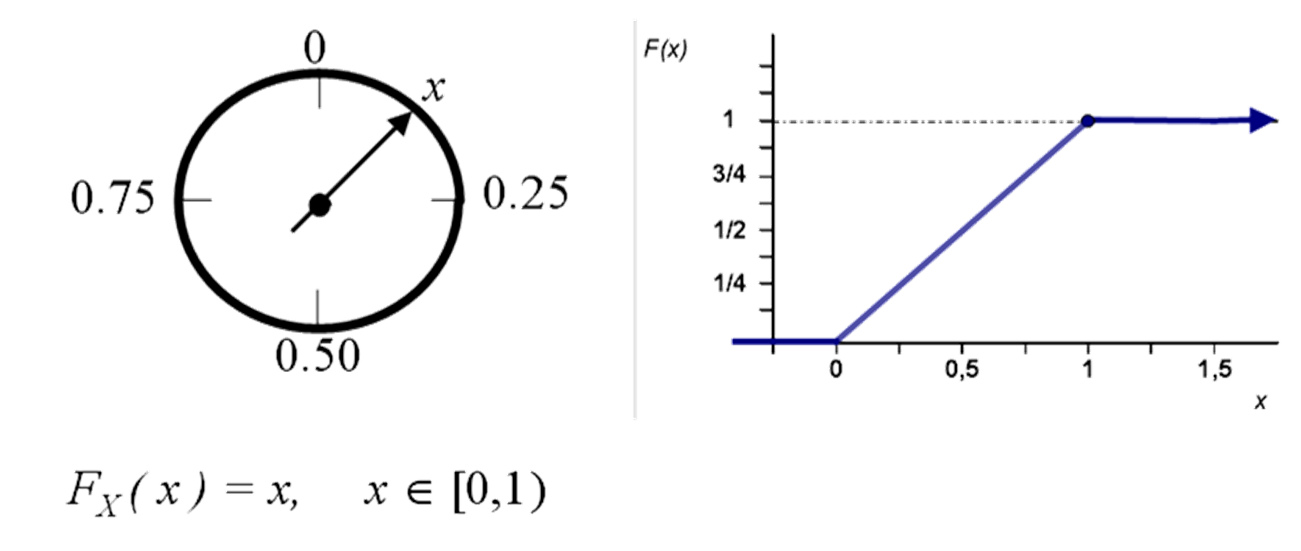
\includegraphics[scale=0.5]{ilustraciones/14.png} 
%ilustracion14%
\end{frame}

\begin{frame}{Función de distribución acumulada}
Si $X$ es una variable aleatoria, la Funci\'on de Distribuci\'on Acumulada mide la probabilidad de un suceso en un intervalo de valores:
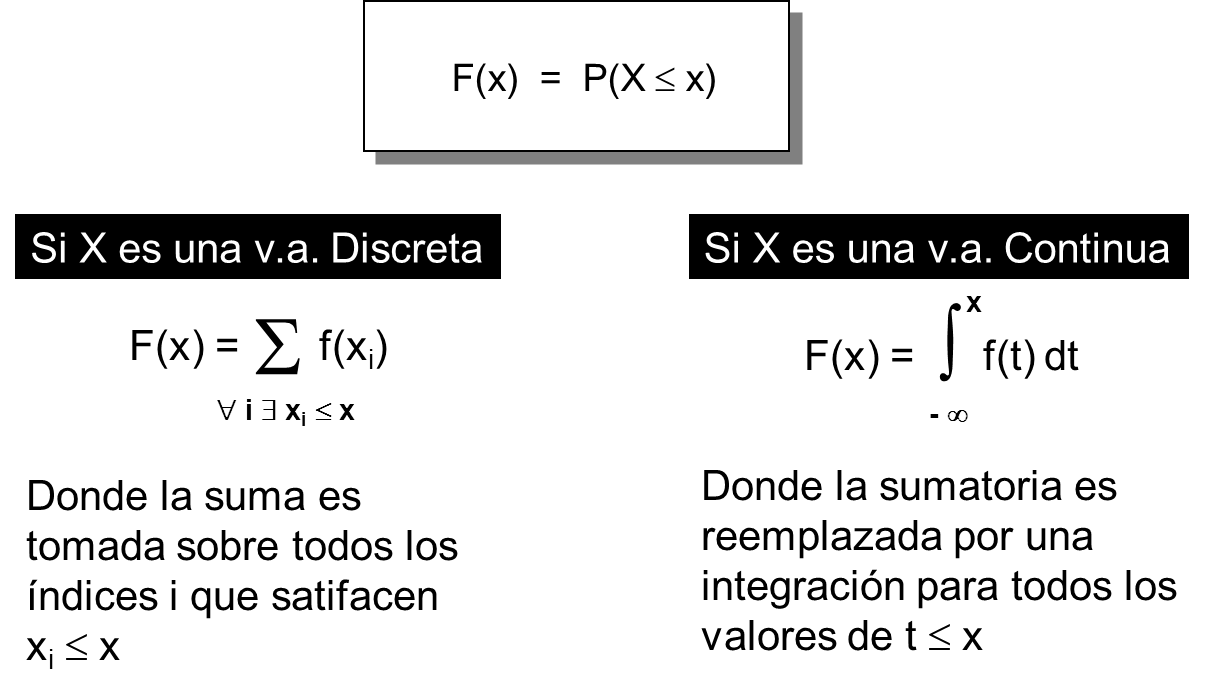
\includegraphics[scale=.5]{ilustraciones/15.png} 
%ilustracion15%
\end{frame}

\begin{frame}{Funci\'on de Probabilidad y de Distribuci\'on Acumulada.}
\begin{center}
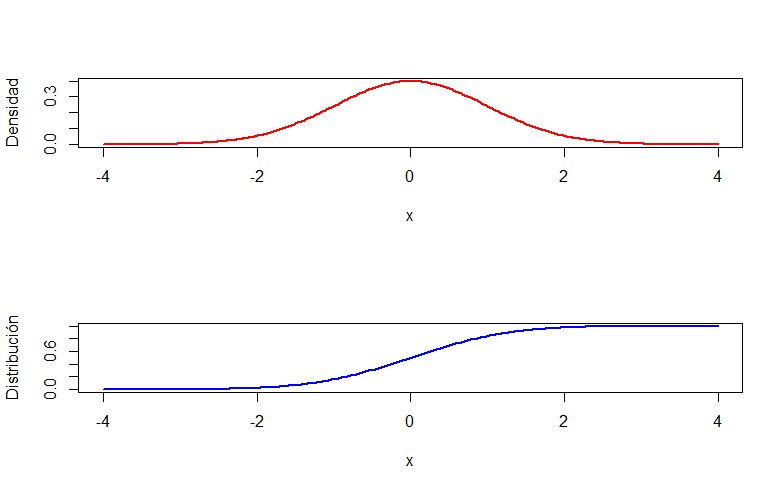
\includegraphics[scale=0.5]{ilustraciones/16.png} 
%ilustracion16%
\end{center}

\end{frame}

\begin{frame}{Funci\'on de Probabilidad y de Distribuci\'on Acumulada.}
\begin{center}
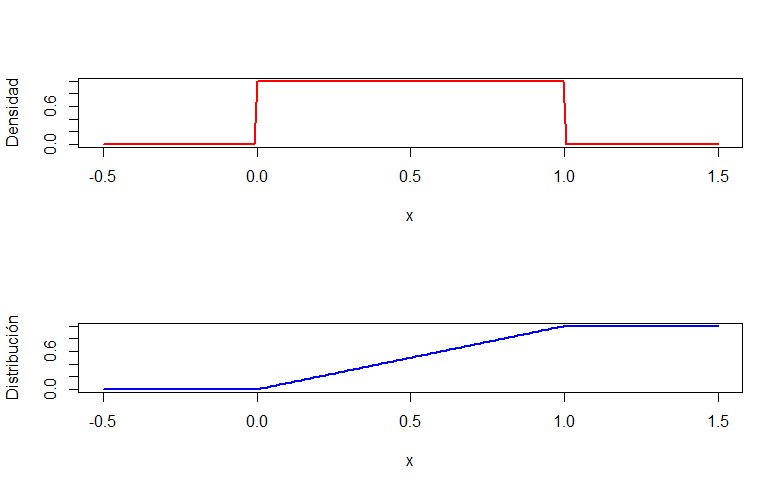
\includegraphics[scale=0.4]{ilustraciones/17.png} 
%ilustracion17%
\end{center}

Función de densidad $f(x)=1$, $x\in [0,1]$

Función de distribución $F(x)=x$, $x\in [0,1)$
\end{frame}

\begin{frame}{Ejemplo de v.a. continua}
Consideremos la variable aleatoria $X$ que representa el tiempo de vuelo de un avi\'on que va de Chicago a Nueva York. Supongamos que el tiempo de vuelo puede ser cualquier valor en el intervalo de 120 a 140 minutos.
Como la variable aleatoria  puede tomar cualquier valor en ese intervalo, $X$ es una variable aleatoria continua y no discreta.
\end{frame}

\begin{frame}{Valor Esperado o Esperanza Matem\'atica}
El valor esperado de una variable aleatoria esta definida por:

$$E(X)=\int _{ -\infty  }^{ \infty  }{ xf\left( x \right) dx } $$

si $x$ es continua, y se le denota por: $E(X)=\mu $

En general, el valor esperado de una función $g(x)$ de la variable aleatoria $X$, está dada por:

$$E(G\left( X \right) )=\int _{ -\infty  }^{ \infty  }{ G\left( x \right)f\left( x \right) dx }$$ si $x$ es continua
\end{frame}

\begin{frame}{Ejemplo de c\'alculo de valor esperado}
\begin{eqnarray*}
f( x ) &=& \left\{ \begin{array}{rl} \frac { 1 }{ b-a } & \mbox{cuando } a \le x\le b \\ 0 & \mbox{en cualquier otro lado} \end{array} \right. \\
E(X) &=& \int _{ -\infty  }^{ \infty  }{ xf( x ) dx } =\int _{ a }^{ b }{ \frac { x }{ b-a } dx } \\
E(X) &=& \frac { 1 }{ b-a } \int _{ a }^{ b }{ xdx } =\frac { 1 }{ b-a } { { \left. \frac { { x }^{ 2 } }{ 2 }  \right|^{b}_{a} }  } \\
E(X) &=& \frac { 1 }{ b-a } \frac { \left( { b }^{ 2 }-{ a }^{ 2 } \right)  }{ 2 } =\frac { a+b }{ 2 }
\end{eqnarray*}
\end{frame}

\begin{frame}{Ejemplo de c\'alculo de valor esperado}

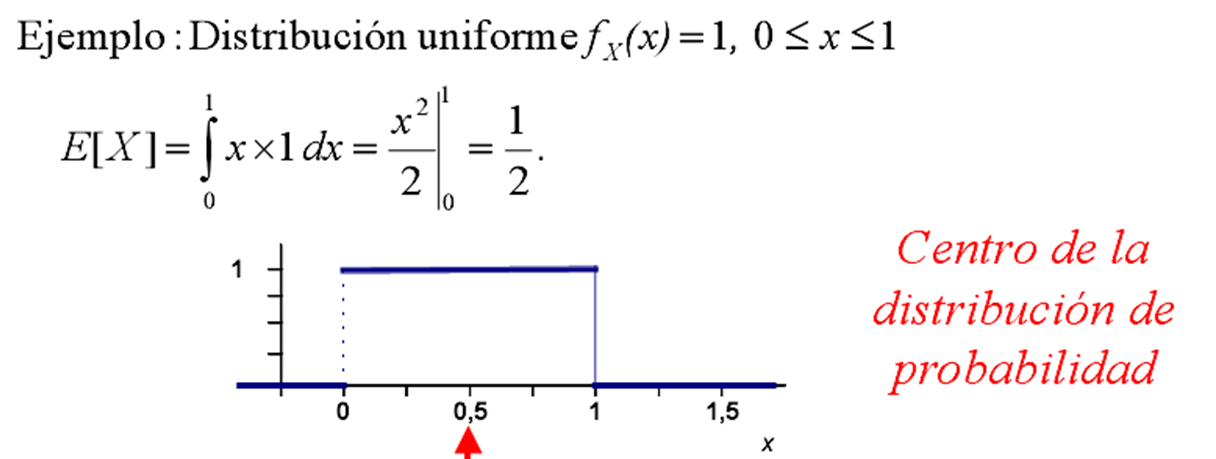
\includegraphics[scale=0.35]{ilustraciones/18.png} 
%ilustracion18%
\end{frame}

\begin{frame}{Varianza}

$$Var(X)=E{ (X-E(X)) }^{ 2 }$$

Por lo que la varianza de una variable aleatoria continua es:

$$Var(X)={ { \sigma  }^{ 2 } }=\int _{ -\infty  }^{ \infty  }{ { (x-\mu ) }^{ 2 } } f\left( x \right) dx$$

Para el ejemplo anterior:

$$Var(X)={ { \sigma  }^{ 2 } }=\int _{ a }^{ b }{ \frac { { (x-\mu ) }^{ 2 } }{ b-a }  } dx=\frac { { (b-a) }^{ 2 } }{ 12 } $$
\end{frame}


\begin{frame}{Propiedades de la varianza}

\begin{enumerate}
	\item $Var(X)=E\left[ { \left( X-\mu  \right)  }^{ 2 } \right] =E\left[ { X }^{ 2 } \right] -{ \mu  }^{ 2 }$


\item $Var(aX+b)={ a }^{ 2 }Var(X)$	
\end{enumerate}
\end{frame}

\begin{frame}{Ejemplos de varianza}

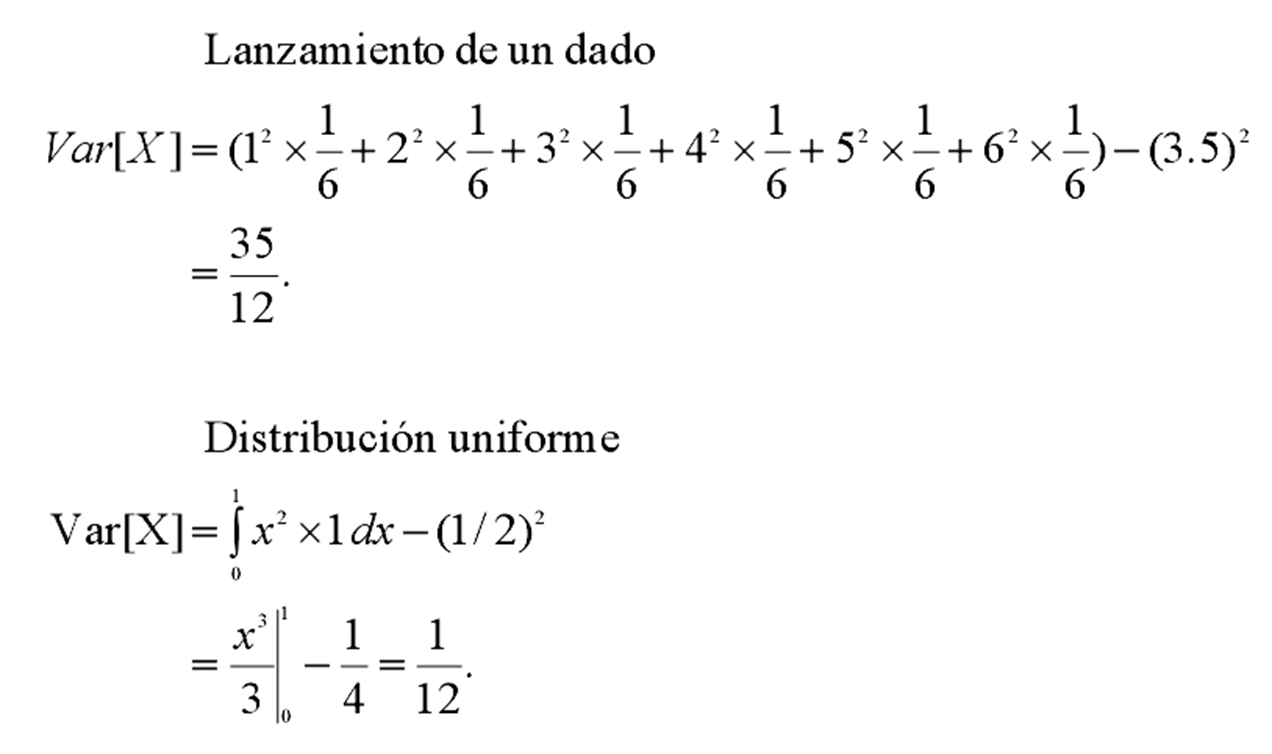
\includegraphics[scale=0.5]{ilustraciones/19.png} 
%ilustracion19%
\end{frame}

\section{Distribución Uniforme Contínua}


\begin{frame}{Uniforme Continua}
Una variable aleatoria $X$  tiene una {\it distribución uniforme} en el intervalo $[a,b]$ si para cualquier intervalo $I$ contenido en $[a,b]$ se tiene que $P(X \in I)$ es proporcional a la longitud de $I$. Usaremos la notación $X \sim U[a,b]$
\begin{eqnarray*}
f( x ) &=& \left\{ \begin{matrix} \frac { 1 }{ b-a } & \mbox{cuando } a\le x\le b \\ 0 & \mbox{en cualquier otro lado} \end{matrix} \right. \\
F( x ) &=& \left\{ \begin{matrix} \frac { x-a }{ b-a } & \mbox{cuando } a\le x\le b \\ 0 & x<a \\ 1 & x>b \end{matrix} \right. \\
E(X) &=& \frac{a+b}{2} \\
Var(X) &=& \frac{ (b-a)^{2}}{12} 
\end{eqnarray*}
\end{frame}

\begin{frame}{Uniforme Continua}
Si $X \sim U[a,b]$ 

\begin{columns}
\column{.45\textwidth}
\begin{block}{$F(x)$}
si $a < x \le b$,
\begin{eqnarray*}
F( x ) &=&  P(X \le x)  \\
       &=& \int_{a}^{x}{\frac{1}{b-a}du} \\
       &=& \left[ \frac{u}{b-a}\right]_a^x \\
       &=& \frac{x-a}{b-a} \\
\end{eqnarray*}

\end{block}
\column{.45\textwidth}
\begin{block}{$E(X)$}
\begin{eqnarray*}
E(X ) &=& \int_{a}^{b}{\frac{1}{b-a} \cdot x\cdot dx} \\
       &=& \left[ \frac{x^2}{2(b-a)}\right]_a^b \\
       &=& \frac{b^2 -a^2}{2(b-a)}  \\
       &=& \frac{a+b}{2} 
\end{eqnarray*}
\end{block}
\end{columns}
\end{frame}
\begin{frame}{Uniforme Continua}
Si $X \sim U[a,b]$ 
\begin{columns}
\column{.45\textwidth}
\begin{block}{$E(X^2)$}
\begin{eqnarray*}
 E(X^2) &=&\int_{a}^{b}{\frac{1}{b-a} \cdot x^2\cdot dx}\\
 &=&  \left[ \frac{x^3}{3(b-a)}\right]_a^b \\
&=& \frac{b^3 -a^3}{3(b-a)} \\
&=& \frac{b^2 + ab + a^2}{3}
\end{eqnarray*}
\end{block}
\column{.55\textwidth}
\begin{block}{$Var(X)$}
\begin{eqnarray*}
&& Var(X) = E(X^2)-E(X)^2 \\
&=& \frac{b^2 + ab + a^2}{3} -  \left(\frac{a+b}{2} \right)^2 \\
&=&  \frac{b^2 + ab + a^2}{3} -  \frac{a^2 +2ab+b^2}{4} \\
&=& \frac{a^2 + 2ab + b^2}{12} \\
&=& \frac{(b-a)^2}{12}
\end{eqnarray*}
\end{block}
\end{columns}


\end{frame}

\begin{frame}{Uniforme Continua}
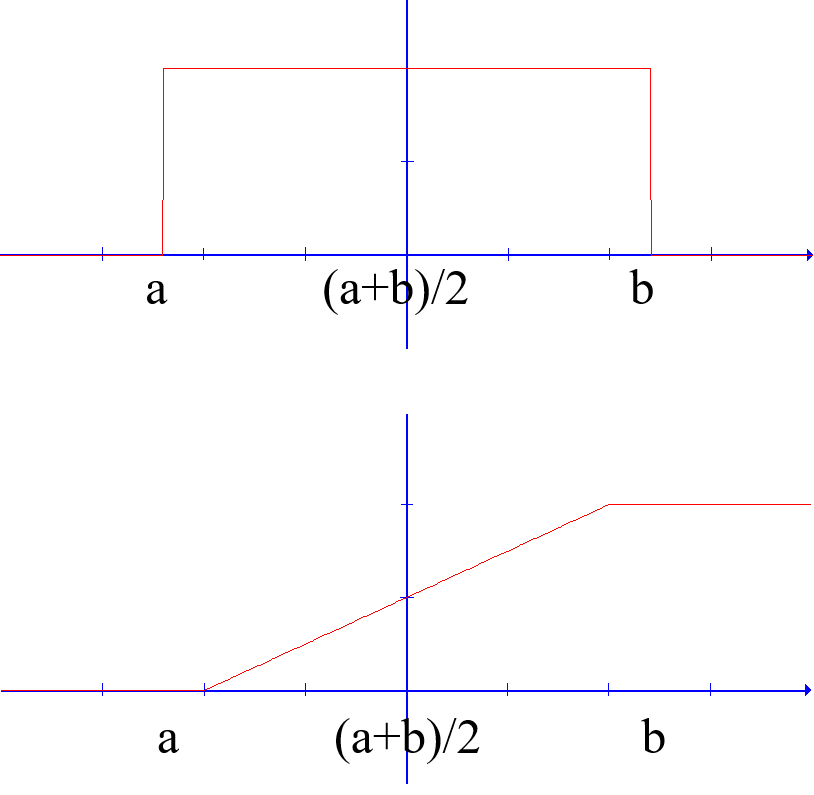
\includegraphics[scale=0.5]{ilustraciones/21.png} 
%ilustracion21%
\end{frame}

\begin{frame}{Uniforme Continua}
\begin{center}
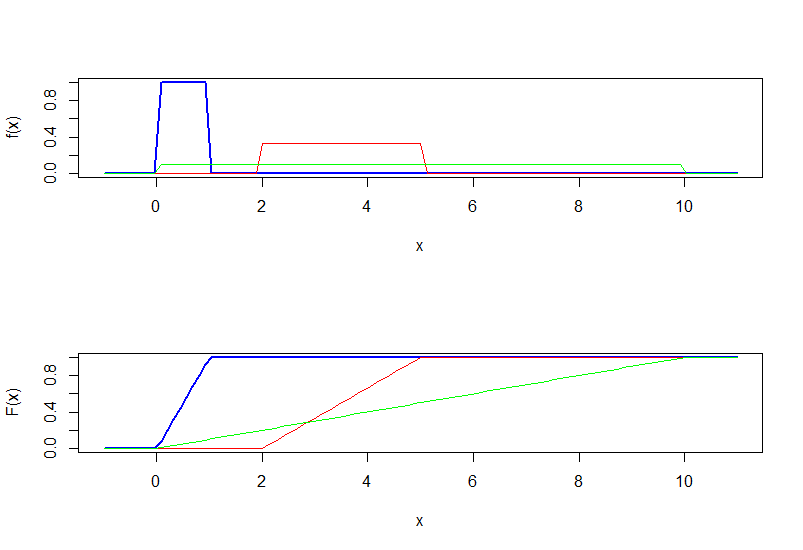
\includegraphics[scale=0.5]{ilustraciones/22.png} 
%ilustracion22%
\end{center}
\end{frame}


\begin{frame}{Ejemplo de v.a. Uniforme Continua}
Consideremos la variable aleatoria X que representa el tiempo de vuelo de un avi\'on que va de Chicago a Nueva York. Supongamos que el tiempo de vuelo puede ser cualquier valor en el intervalo de 120 a 140 minutos.

Supongamos que tenemos suficientes dato reales para suponer que cualquier intervalo de un minutos entre 120 y 140 es igualmente probable, entonces la variable aleatoria X  tiene una distribución uniforme de probabilidades y
\end{frame}

\begin{frame}{Ejemplo de v.a. Uniforme Continua}

\begin{eqnarray*}
f( x ) &=& \left\{ \begin{matrix} \frac { 1 }{ 20 } & \mbox{cuando } 120 \le x\le 140 \\ 0 & \mbox{en cualquier otro lado} \end{matrix} \right. \\
F( x ) &=& \left\{ \begin{matrix} \frac { x-120 }{20 } & \mbox{cuando } 120 \le x\le 140 \\ 0 & x<140 \\ 1 & x>140 \end{matrix} \right. \\
E(X) &=& 130 \mbox{ minutos}\\
Var(X) &=& 33.33 \\
\sigma &=& 5.77 \mbox{ minutos} \\
\end{eqnarray*}

\end{frame}


\begin{frame}{Ejemplo de v.a. Uniforme Continua}
\begin{enumerate}
\item ¿Cuál es la probabilidad de que el vuelo de Chicago a Nueva York sea de entre  125:00  y 132:00 minutos?
\begin{eqnarray*}
P( 125 \le X \le 132 ) &=&  F(132) - F(125)\\
&=& \frac{132-120 }{20 } -  \frac{125-120 }{20 }   \\
 &=&  \frac{7 }{20 }  \\
\end{eqnarray*}
\item ¿Cuál es la probabilidad de que tarde más de 135:00 minutos? 
\begin{eqnarray*}
P( X \ge 135 ) &=& 1-  F(135) \\
&=& 1  -  \frac{135-120 }{20 }   \\
 &=& \frac{ 5 }{20 }  \\
\end{eqnarray*}
\end{enumerate}
\end{frame}
\section{Distribución Normal}



\begin{frame}{Distribuci\'on Normal o Gaussiana}

La distribuci\'on de probabilidad m\'as importante en el campo de la probabilidad y la estad\'istica es la {\bf distribuci\'on de probabililidad normal}, que tiene funci\'on de densidad de probabilidad (f.d.p.) a

$$f\left( x;\mu ,{ \sigma  }^{ 2 } \right) =\frac { 1 }{ \sqrt { 2\pi { \sigma  }^{ 2 } }  } exp\left( -\frac { { \left( x-\mu  \right)  }^{ 2 } }{ 2{ \sigma  }^{ 2 } }  \right) \mbox{ con }-\infty <x<\infty $$

Donde $\mu$  y ${ \sigma  }^{ 2 }$ son los par\'ametros de la distribuci\'on.

 \bigskip
Si una variable aleatoria (v.a.) $X$ tiene una f.d.p. como la anterior la denotaremos como: $X\sim N(\mu ,{ \sigma  }^{ 2 }) $ 
\end{frame}


\begin{frame}{Distribución Normal}
Si $X\sim N(\mu ,{ \sigma  }^{ 2 }) $  con $-\infty <x<\infty$
\begin{eqnarray*}
f\left( x;\mu ,{ \sigma  }^{ 2 } \right) &=&\frac { 1 }{ \sqrt { 2\pi { \sigma  }^{ 2 } }  } exp\left( -\frac { { \left( x-\mu  \right)  }^{ 2 } }{ 2{ \sigma  }^{ 2 } }  \right)   \\
F( x ) &=& \int_{- \infty}^{x} \frac { 1 }{ \sqrt { 2\pi { \sigma  }^{ 2 } }  } exp\left( -\frac { { \left( u-\mu  \right)  }^{ 2 } }{ 2{ \sigma  }^{ 2 } }   \right) \cdot du  \\
E(X) &=& \mu \\
Var(X) &=& \sigma^2 
\end{eqnarray*}
\end{frame}


\begin{frame}{Propiedades de la Distribuci\'on Normal}
La distribuci\'on es sim\'etrica con respecto a $\mu$, es decir $f( \mu + x) = f( \mu - x)$. Además es unimodal y su moda, mediana y media poseen el mismo valor. 
\begin{center}
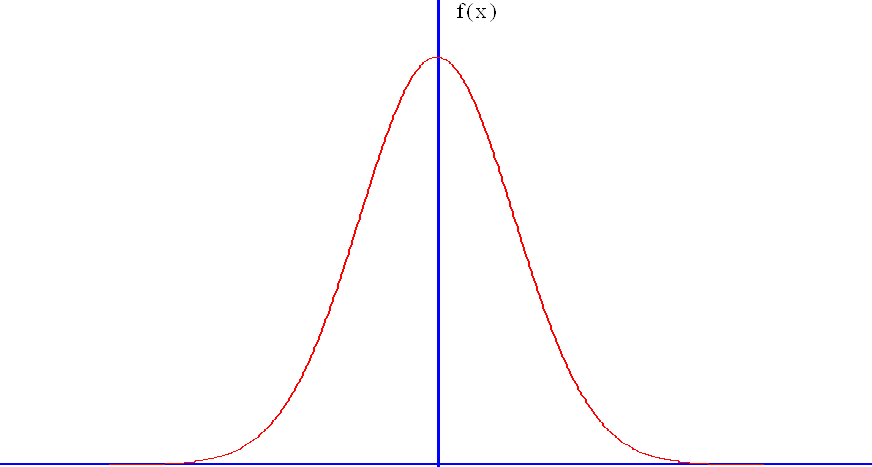
\includegraphics[scale=0.5]{ilustraciones/28.png} 
\end{center}
%ilustracion28%
$$E(X)= \mu \hspace{30pt} Var(X)= \sigma ^2  \hspace{30pt} \sigma_X= \sigma $$
\end{frame}

\begin{frame}

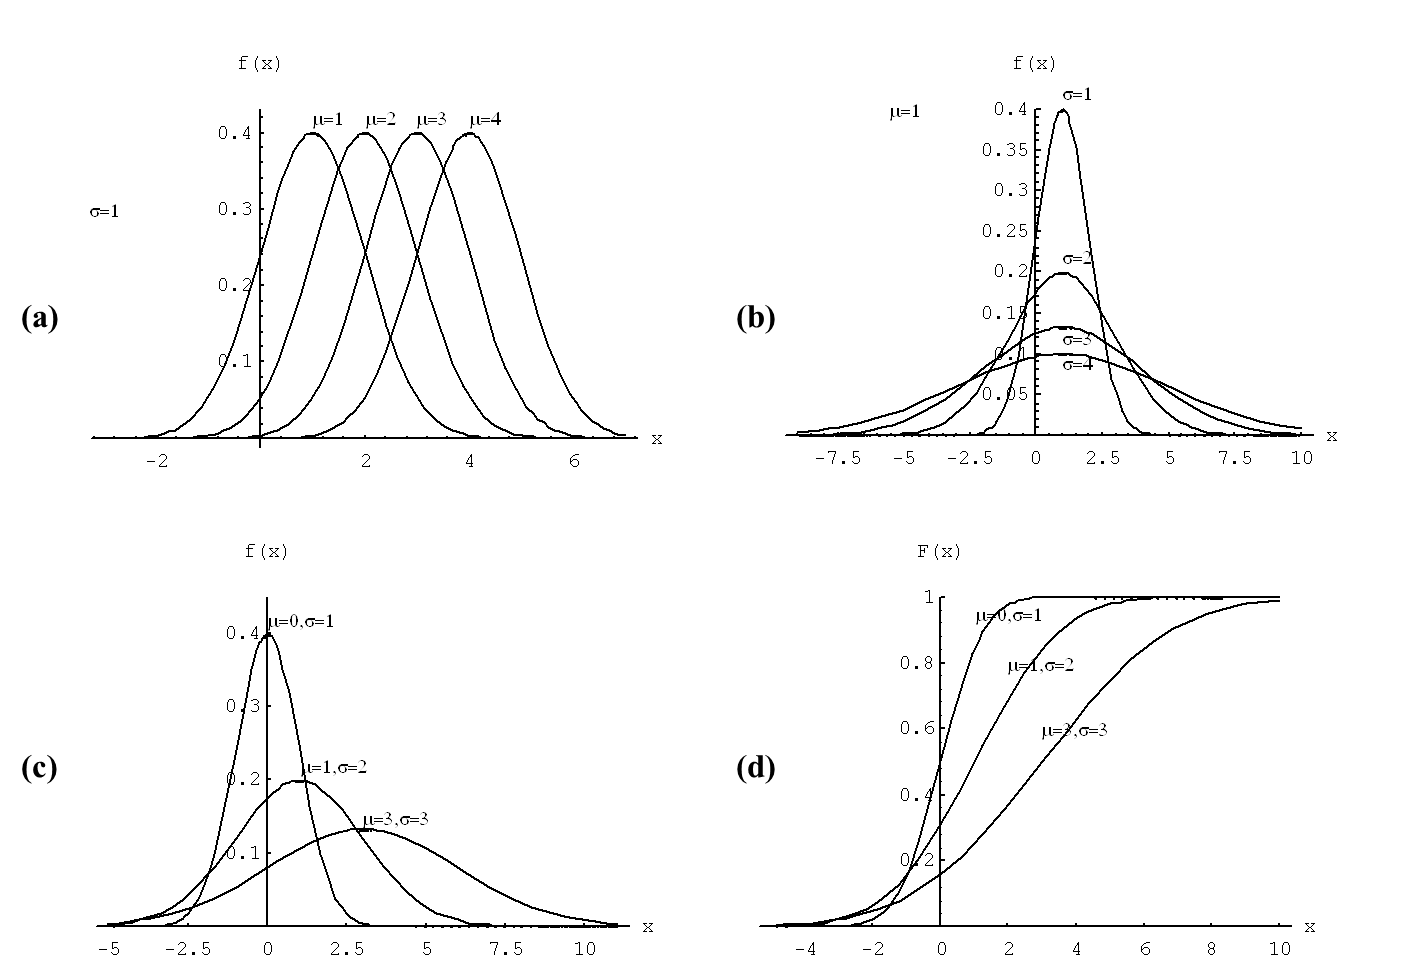
\includegraphics[scale=0.45]{ilustraciones/27.png} 
%ilustracion27%
\end{frame}


\begin{frame}{Propiedades de la Distribuci\'on Normal}
Aunque la v.a. X puede tomar cualquier valor entre $-\infty $ y $+\infty $

\bigskip
Aprox. 68\% de la dist. está en el intervalo $\mu \pm \sigma $

Aprox. 95\% de la dist. está en el intervalo $\mu \pm 2\sigma $

Aprox. 99\% de la dist. está en el intervalo $\mu \pm 3\sigma $

\bigskip
o equivalentemente

$$P\left[ \mu -\sigma <X<\mu +\sigma  \right] =0.683$$

$$P\left[ \mu -2\sigma <X<\mu +2\sigma  \right] =0.954$$

$$P\left[ \mu -3\sigma <X<\mu +3\sigma  \right] =0.997$$
\end{frame}

\begin{frame}
\begin{center}
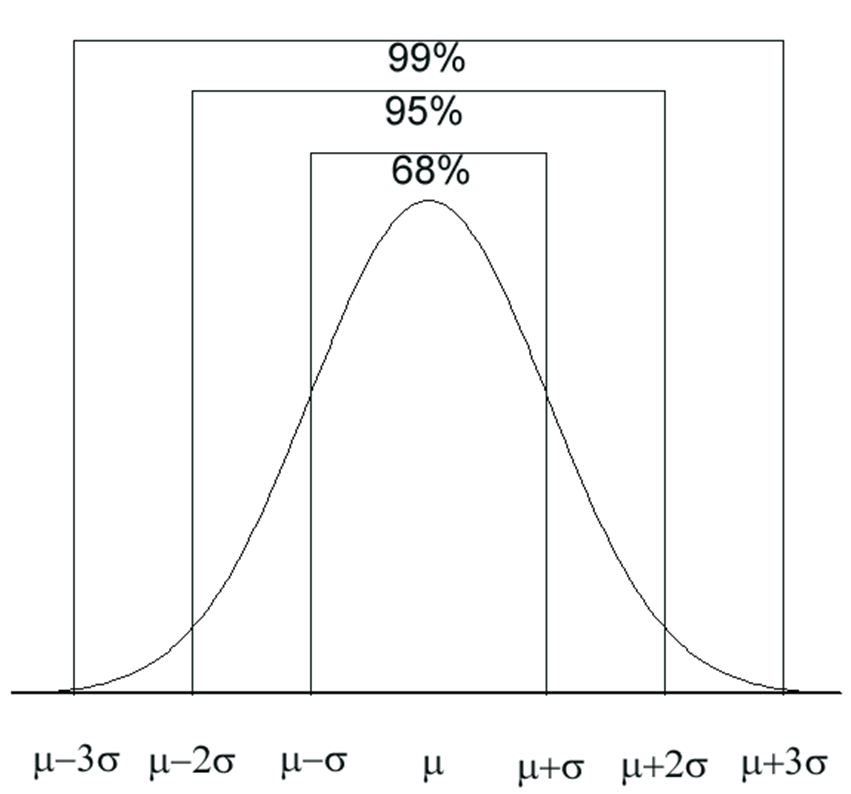
\includegraphics[scale=0.5]{ilustraciones/30.png} 
%ilustracion30%
\end{center}
\end{frame}


\begin{frame}{Distribuci\'on Normal Est\'andar}

La distribuci\'on con media $ \mu =0$ y varianza $ { \sigma  }^{ 2 }=1$ se llama Distribuci\'on Normal Est\'andar
$$f\left( z \right) =\frac { 1 }{ \sqrt { 2\pi  }  } exp\left( -\frac { { z }^{ 2 } }{ 2 }  \right) ,\quad -\infty <z<\infty $$
Usualmente se denota la v.a. normal est\'andar por Z. Entonces lo denotamos como 
$Z\sim N\left( 0,1 \right) $
\end{frame}

\begin{frame}
\begin{center}
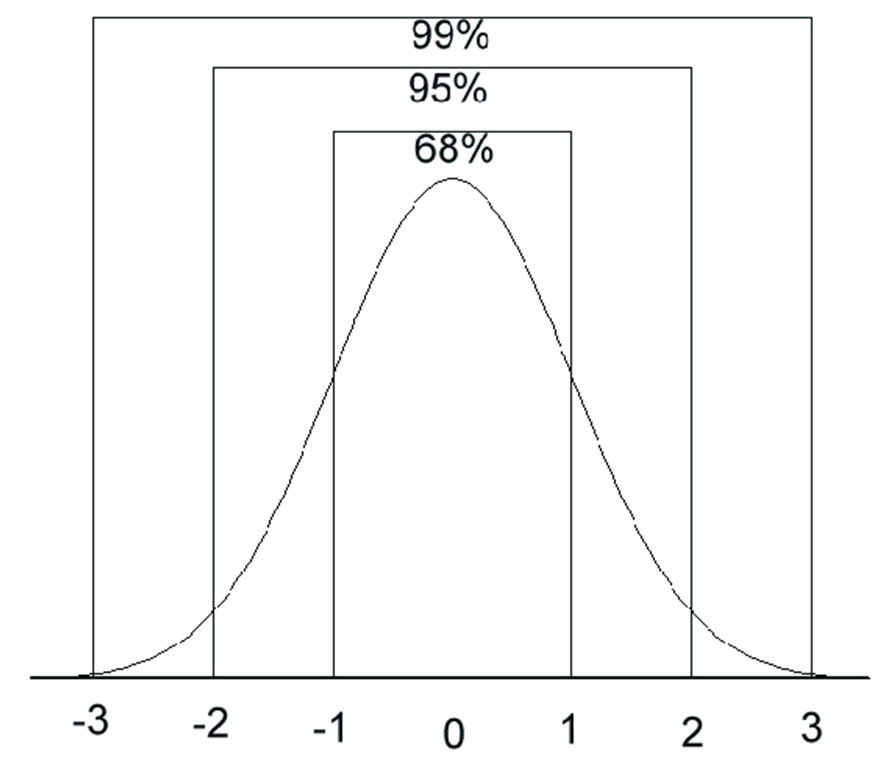
\includegraphics[scale=0.5]{ilustraciones/31.png} 
%ilustracion31%
\end{center}
\end{frame}

\begin{frame}

Para determinar \'areas bajo esta curva nos basamos en la tabla que tiene tabulados la funci\'on de distribuci\'on acumulativa de $Z$, esto es,
$P\left( Z\le z \right) =\Phi (z)$
\begin{center}
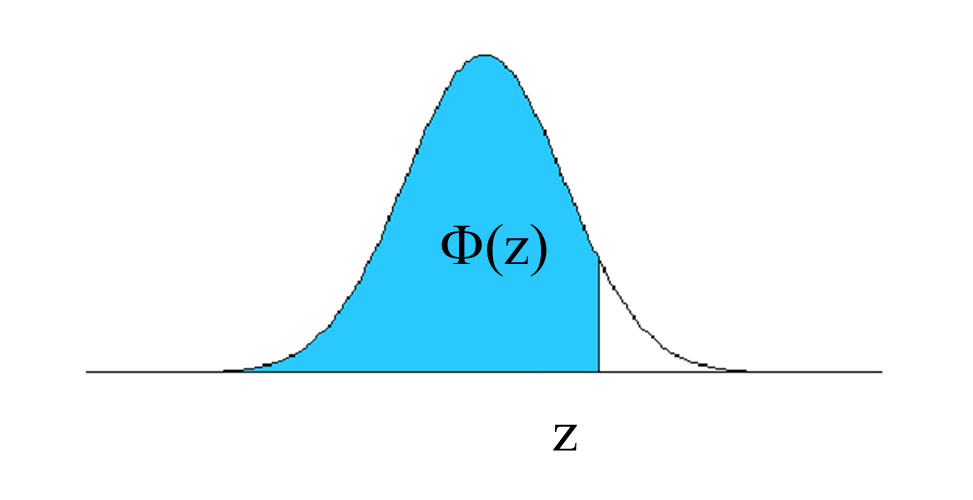
\includegraphics[scale=.5]{ilustraciones/32.png} 

%ilustracion32%
\end{center}
\end{frame}

\begin{frame}
Usando dicha tabla determinamos probabilidades correspondientes a valores espec\'ificos de $z$.

1)$P\left( Z<1.96 \right) =\Phi (1.96)=0.975$
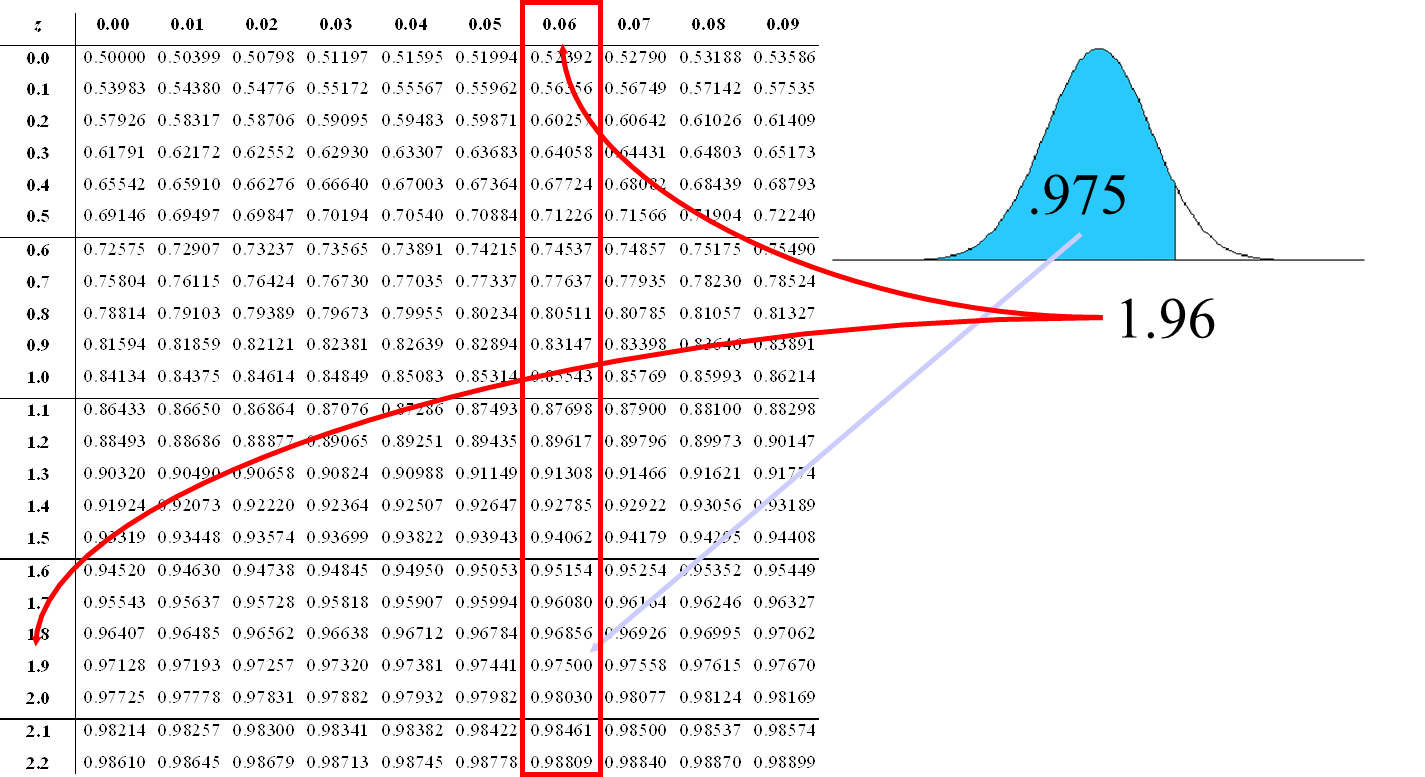
\includegraphics[scale=0.5]{ilustraciones/33.png} 
%ilustracion33%
\end{frame}

\begin{frame}

2) $P\left( Z\ge 1.96 \right)=1-P(Z<1.96)=1-\Phi (1.96)=1-0.975=0.025$
\begin{center}
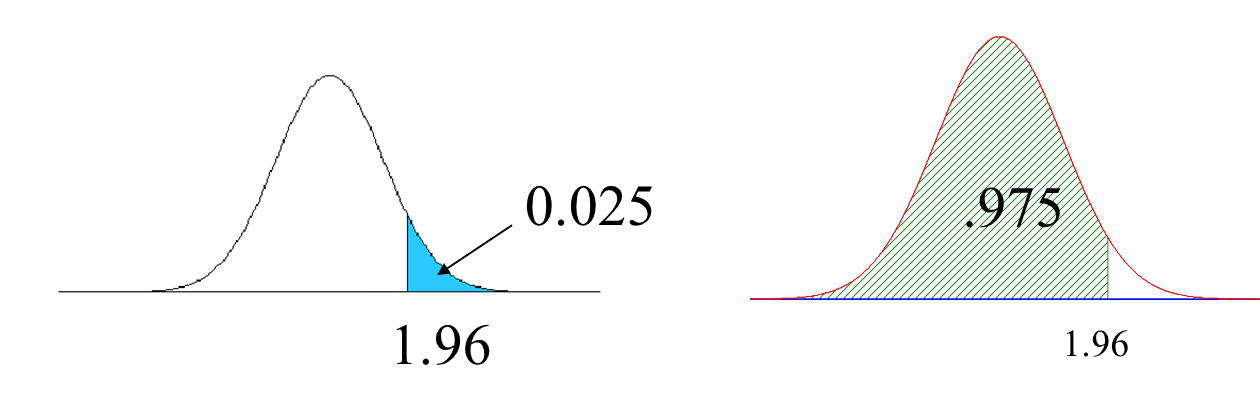
\includegraphics[scale=0.5]{ilustraciones/34.png} 
\end{center}
%ilustracion34%
\end{frame}

\begin{frame}
3) $P\left( -1.96<Z<2.31 \right) =\Phi (2.31)-\Phi (-1.96) =0.9896-0.025=0.9643$
\begin{center}
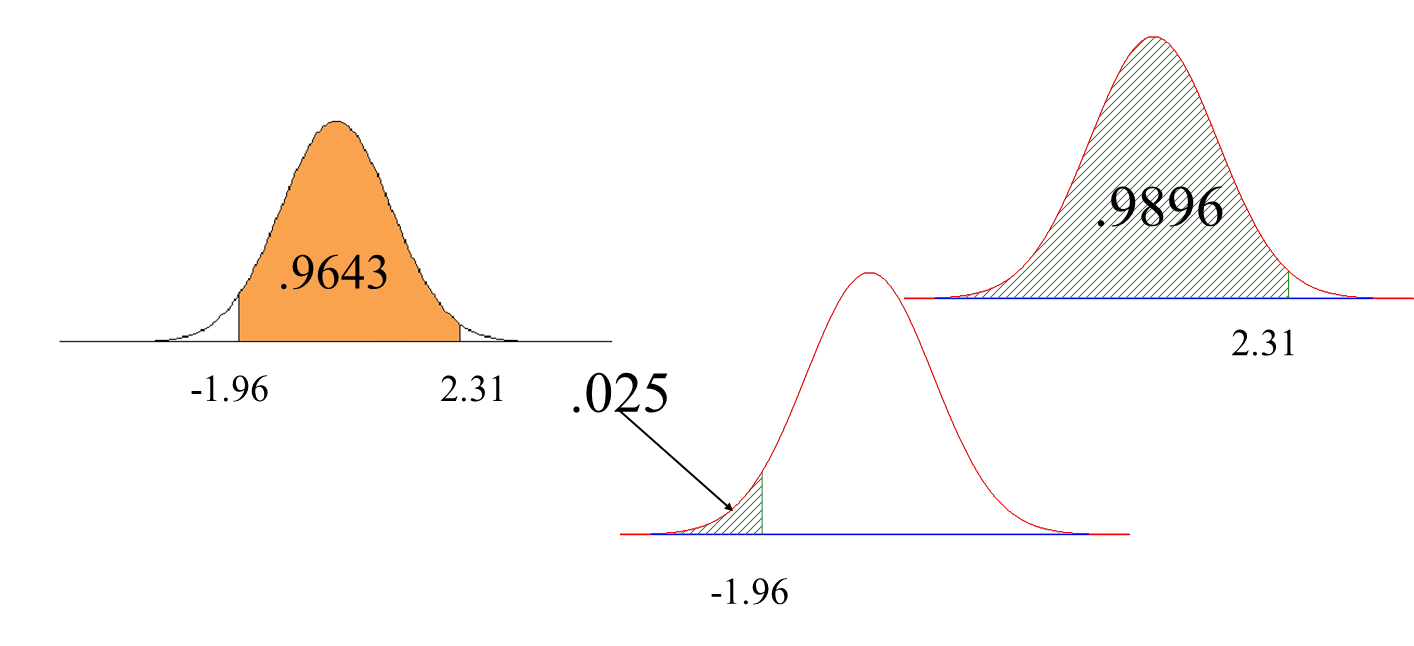
\includegraphics[scale=0.5]{ilustraciones/35.png} 
%ilustracion35%							
\end{center}
\end{frame}

\begin{frame}
4)  $P\left( 1.96<Z<2.31 \right) =\Phi (2.31)-\Phi (1.96)=0.9896-0.975=0.0146$
\begin{center}
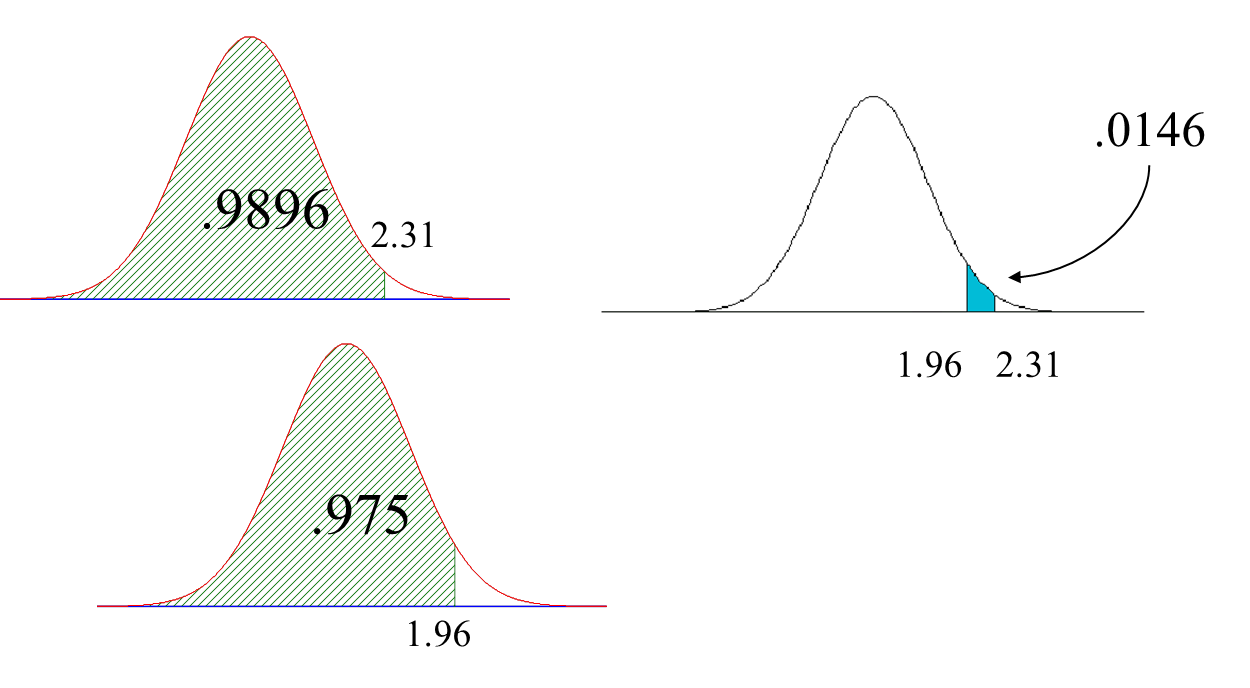
\includegraphics[scale=0.5]{ilustraciones/36.png} 
%ilustracion36%							
\end{center}
\end{frame}

\begin{frame}{Cuantiles}

Por otra parte nos puede interesar determinar z cuando hemos determinado de antemano la probabilidad, por ejemplo:

1) Determine z tal que $P(Z>z)=0.2483$
Respuesta: Como el área total bajo la curva es uno,

$$P(Z\le z)=1 - P(Z>z)=1-0.2483=0.7517$$

entonces

$$\Phi (z)=0.7517$$
\end{frame}

\begin{frame}
\begin{center}
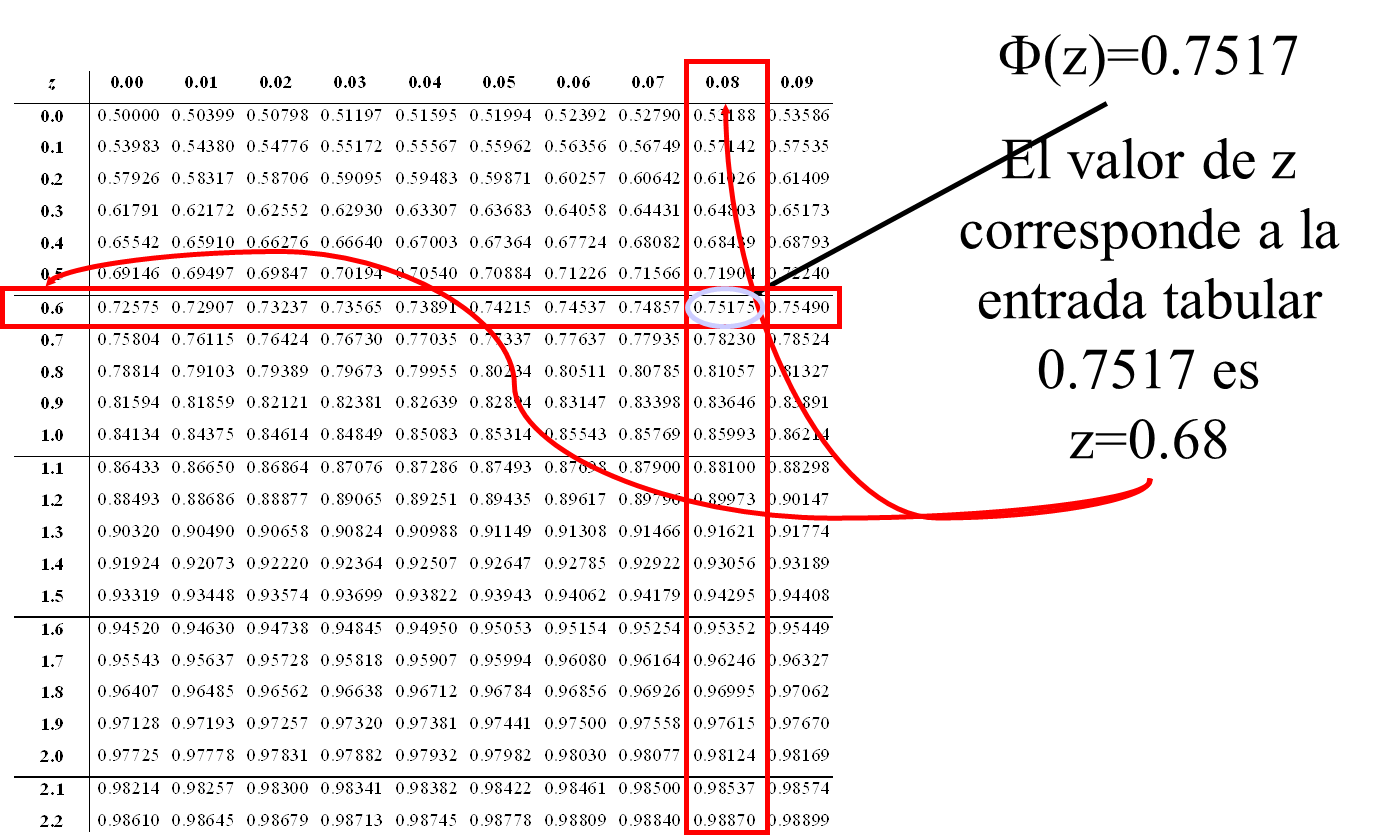
\includegraphics[scale=0.5]{ilustraciones/37.png} 
%ilustracio37%
\end{center}
\end{frame}

\begin{frame}
2) Obtener el valor de $z>0$ de tal forma que 

$$P(-z<Z<z)=0.90$$

Respuesta: Por la simetr\'ia de la distribuci\'on tenemos que

$$P(Z<z) = P(Z>z) = 0.05$$
\begin{center}
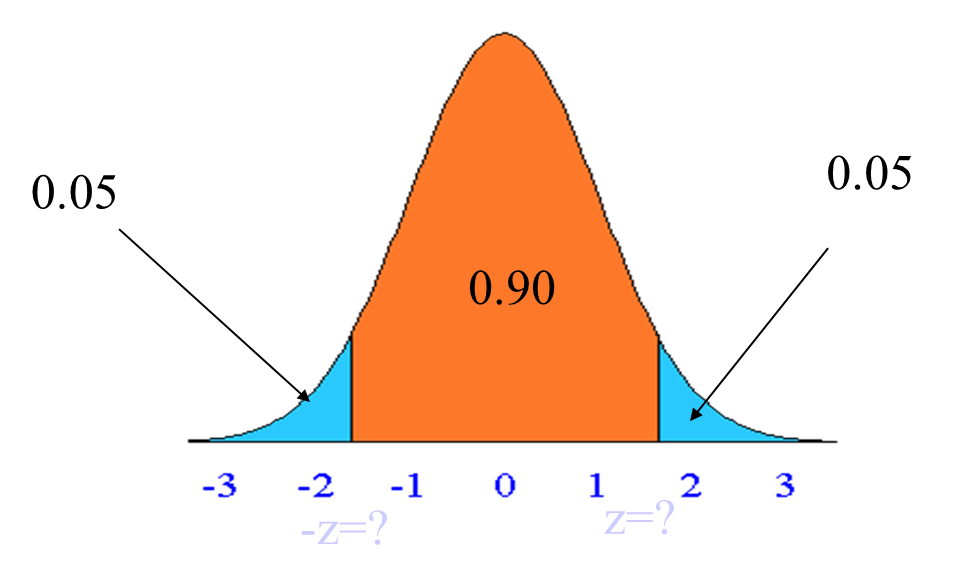
\includegraphics[scale=0.5]{ilustraciones/38.png} 
%ilustracio38%
\end{center}
\end{frame}

\begin{frame}
De la tabla tenemos que $\Phi (1.64)=0.9495$ y $\Phi (1.65)=0.9505$. Entonces $z$ está entre $1.64$ y $1.65$. As\'i que $z=1.645$.
\begin{center}
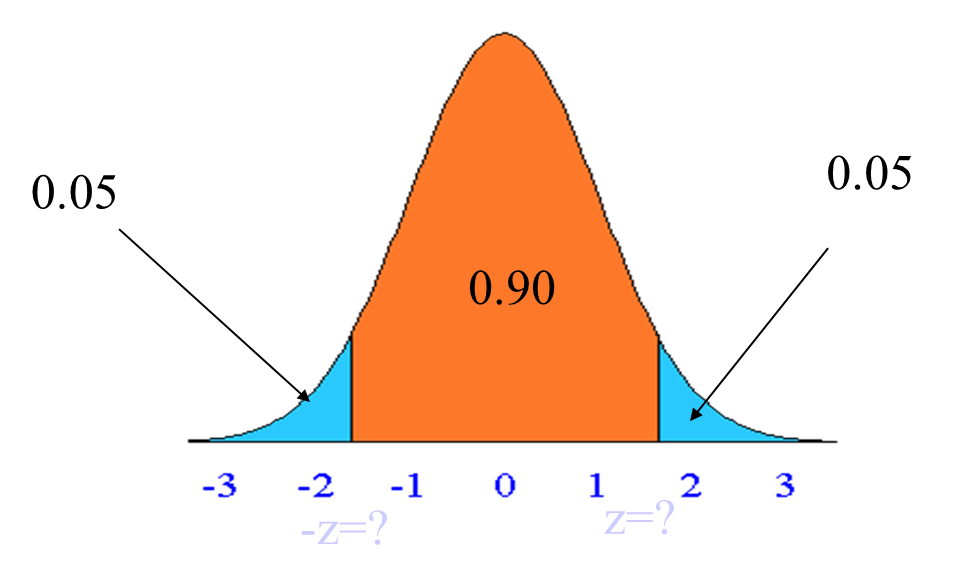
\includegraphics[scale=0.5]{ilustraciones/38.png} 
%ilustracio38%
\end{center}
\end{frame}

\begin{frame}{Estandarizando una Variable Normal}
Si $X\sim N(\mu ,{ \sigma  }^{ 2 })$ para calcular la probabilidad de algunos valores de $X$ de manera \textit{f\'acil}, primero estandarizamos $X$.

\bigskip
Si especificamos  $\mu $ y ${ \sigma  }^{ 2 }$ , entonces

$$Z=\frac{(X-\mu )}{\sigma} \sim N(0,1)$$
\end{frame}

\begin{frame}{Ejemplo}
 Ejemplo: Supongamos $X\sim N(50,4)$, entonces determine $P(48<X<53)$.

\bigskip
Respuesta: Primero estandarizamos $X$, para obtener una variable $X\sim N(0,1)$
\begin{eqnarray*}
P[48<X<53]&=&P\left[\frac{(48-50)}{2}<\frac{(X-\mu )}{\sigma} <\frac{(53-50)}{2}\right] \\
		  &=&P\left[\frac{(48-50)}{2}<Z<\frac{(53-50)}{2}\right] \\
		  &=&P[-1<Z<1.5]
\end{eqnarray*}		  
\end{frame}

\begin{frame}
\begin{center}
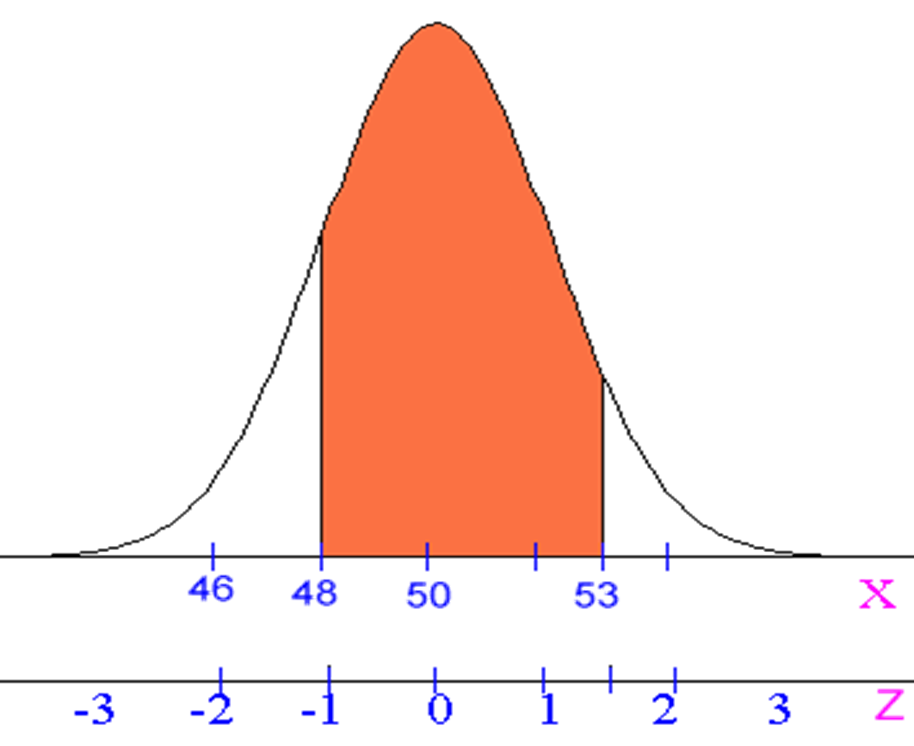
\includegraphics[scale=0.5]{ilustraciones/39.png} 
%ilustracion39%
\end{center}
\end{frame}

\begin{frame}{Ejemplo}

La longitud $X$ de ciertos tornillos es una variable aleatoria con distribuci\'on normal de media $30 mm$ y desviaci\'on t\'ipica $0.2 mm$. Se aceptan como v\'alidos aquellos que cumplen
 
$$29.5 < X < 30.4$$
Calcular:
\begin{enumerate}
\item Proporci\'on de tornillos no aceptables por cortos.

\item Proporci\'on de tornillos no aceptables por largos.

\item Proporci\'on de tornillos no v\'alidos.
\end{enumerate}
\end{frame}


\begin{frame}{Ejemplo (soluci\'on)}
$$X \sim N(30, .04) \Rightarrow Z=\frac{X- \mu}{\sigma} \sim N(0,1)$$
1.
\begin{eqnarray*}
P(X \le 29.5) &=& P\bigg(\frac{X-30}{0.2} \le \frac{29.5-30}{0.2} \bigg) \\
&=& P(Z \le -2.5) = \Phi(-2.5) = 0.0068 
\end{eqnarray*}
\begin{center}
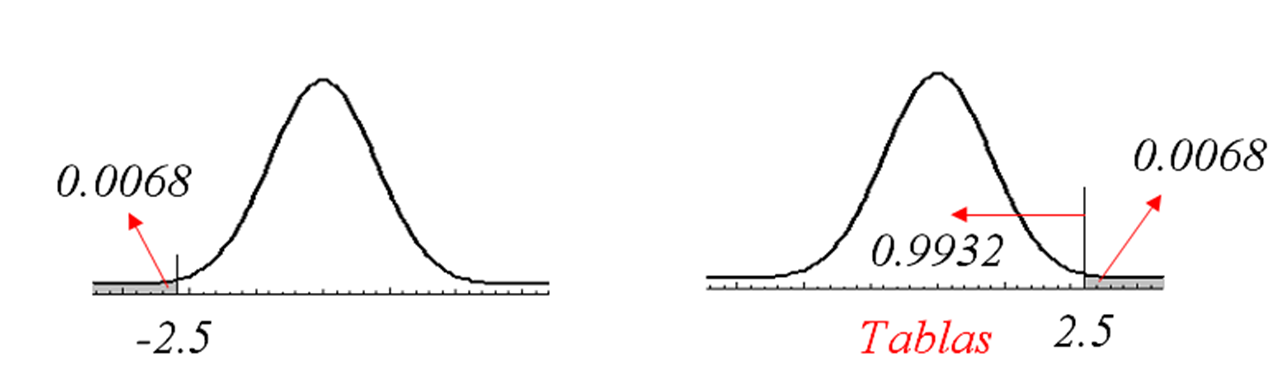
\includegraphics[scale=0.3]{ilustraciones/40.png} 
%ilustracion40%
\end{center}
\end{frame}

\begin{frame}{Ejemplo (soluci\'on)}
2. 
\begin{eqnarray*}
P(X \ge 30.4) &=& P\bigg(\frac{X-30}{0.2} \ge \frac{30.4-30}{0.2} \bigg) \\
&=& P(Z \ge 2) =1- \Phi(2) = 0.0228
\end{eqnarray*}
3.
\begin{eqnarray*}
P(\mbox{`'Defectuosas''}) &=& 0.0228+0.0068 = 0.0296 \\
Y &=& \mbox{No. de piezas defectuosas en un lote de 1,000} \\
E[Y] &=& 1000 \times 0.0296 =29.6
\end{eqnarray*}

\end{frame}


\begin{frame}{Ejemplo}

La longitud de los clavos fabricados por una m\'aquina, en mil\'imetros, es una variable aleatoria $X$ que sigue una distribuci\'on normal, con media $10$ y varianza $4$. Se debe dar una especificaci\'on del m\'aximo de  la longitud de los clavos, tal que el 90\% de los clavos cumpla con la especificaci\'on. ¿Cu\'al debe ser la especificaci\'on?

\end{frame}

\begin{frame}{Ejemplo}

Tenemos $X\sim N(10;4)$ y adem\'as nos piden que $P\left( X\le x \right)=0.9$ entonces  $F(x)=0.9$
por lo que $\Phi (\frac{x-10}{2})=0.9$ por lo tanto $\frac{x-10}{2}=z_{0.9}$.

\bigskip
Usamos la tabla y obtenemos que
$\Phi (1.28)=0.9$.

\bigskip
 Entonces $\frac{x-10}{2}=1.28$ así que $x=12.56$

\bigskip
Con lo cual si decimos que la longitud m\'axima de los clavos debe ser de 12.56 el $90\%$ de los clavos fabricados cumplir\'a con la especificaci\'on
\end{frame}

\begin{frame}{Encontrar los par\'ametros}
Otro problema posible es que sepamos que una variable aleatoria es normal pero no conozcamos los par\'ametros $\mu$ y $\sigma$. Si conoci\'eramos, por ejemplo, para 2 valores $x_1$ y $x_2$ que la probabilidad de que $X$ sea menor o igual a esos valores es p1 y p2 respectivamente, entonces podremos calcular el valor de los par\'ametros, es decir, la forma que la campana debe tener para que $P(X{ \le x }_{ 1 })={ p }_{ 1 }$ y $P(X{ \le x }_{ 2 })={ p }_{ 2 } $. Si estandarizamos llegamos a que:
\end{frame}

\begin{frame}{Encontrar los par\'ametros}

$$\Phi \left(\frac{x_1 -\mu}{\sigma}\right) =p_1 \mbox{ y } \Phi \left(\frac{x_2 -\mu}{\sigma} \right) =p_2$$

Conociendo $ { p }_{ 1 }$ y ${ p }_{ 2 } $, de la tabla obtenemos ${ z }_{ p_1 } $ y ${ z }_{ p_2 } $, con lo cual podemos plantear un sistema de 2 ecuaciones con 2 inc\'ognitas, debido a que $ { x }_{ 1 }$ y $ { x }_{ 2 }$ tambi\'en son datos.
$$\left\{\begin{matrix}
\dfrac{x_1 -\mu}{\sigma}=z_{p_1}\\ 
\dfrac{x_2 -\mu}{\sigma}=z_{p_2}
\end{matrix}\right.$$

Y resolviendo el sistema conseguimos $\mu $ y $\sigma $.
\end{frame}

\begin{frame}{Ejemplo}

La longitud de los clavos fabricados por una m\'aquina, en mil\'imetros, es una variable aleatoria X que sigue una distribuci\'on normal. Se sabe que el 80\% de los clavos fabricados miden menos de 10mm, y que el 90\% de los clavos fabricados miden menos de 11mm. ¿Cu\'al es la media y la varianza de los clavos producidos por la m\'aquina?
\end{frame}

\begin{frame}{Soluci\'on}
Sabemos que $P(X\le 10)=0.8 $ y $P(X\le 11)=0.9$. Estandarizamos y nos queda que:
$$\Phi \left(\frac{10 -\mu}{\sigma}\right) =0.8 \mbox{ y } \Phi \left(\frac{11 -\mu}{\sigma} \right) =0.9$$


De la tabla obtenemos que $F(0.8416)=0.8$ y $F(1.2816)=0.9$. Planteamos:
$$\left\{\begin{matrix}
\dfrac{10 -\mu}{\sigma}=0.8416\\ 
\dfrac{11 -\mu}{\sigma}=1.2816
\end{matrix}\right.$$

Resolvemos y obtenemos que $\mu =8.08$ y $\sigma =2.27 $.Es decir: $X\sim N(8.08;2.{ 27 }^{ 2 })$.
\end{frame}

\section{Distribución Ji-cuadrada}


\begin{frame}{Distribuci\'on Ji-cuadrada}
Se dice que $X$ tiene una distribuci\'on Ji-cuadrada  si tiene las siguiente forma:
$$f(t)=\left\{\begin{matrix}
\dfrac{x^{(\nu -2)/2}exp(-x/2)}{2^{\nu/2}\Gamma(\nu/2)} & x>0\\ 
& \\
0 & x\le 0 
\end{matrix}\right.$$
Donde $\nu$ es un n\'umero natural y se conoce con el nombre de \textit{grados de libertad}

\bigskip
$E(X)=\nu \hfill  Var(X)=2\nu $
\end{frame}

\begin{frame}{Función Gama}

$\Gamma \left( x \right) = \int_{0}^{\infty}u^{x-1} e^{-u}du$

\bigskip
Pero en el caso en que x es entero entonces:


\bigskip
$\Gamma \left( x \right) = (x-1)!$

\end{frame}

\begin{frame}{Distribuci\'on Ji-cuadrada}
\begin{center}
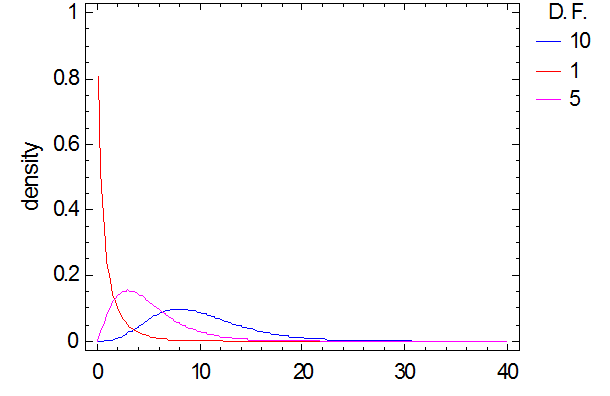
\includegraphics[scale=0.6]{ilustraciones/50.png} 
%ilustracion50%
\end{center}
\end{frame}

\begin{frame}{Distribuci\'on Ji-cuadrada}
\begin{center}
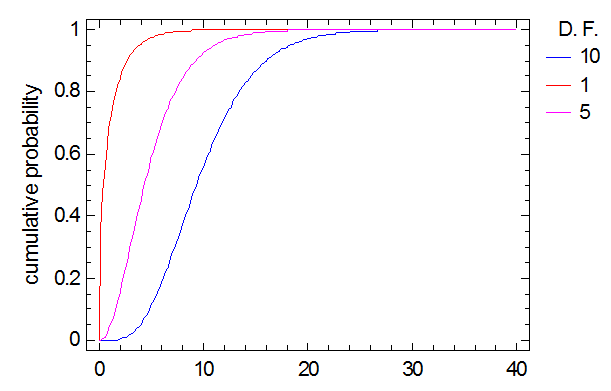
\includegraphics[scale=0.6]{ilustraciones/51.png} 
%ilustracion51%
\end{center}
\end{frame}

\begin{frame}{Utilizaci\'on}
\begin{itemize}

\item Debido al uso que le daremos, lo que nos interesa calcular de la distribuci\'on chi-cuadrada son sus Cuantiles. Es decir, los valores $x$ tales que $P(X \le x)$ es igual a un cierto $\alpha$.

\item Sea $ X\sim { { x }_{ (v) }^{ 2 } }$, ${ x }_{ \alpha ,\nu  }^{ 2 }$, es el valor $x$ tal que $P(X\le x)=\alpha$. Es decir, el valor tal que la probabilidad de que una variable chi-cuadrado con $n$ grados de libertad resulte menor que ese valor sea $\alpha$. Dicho de otra forma, el valor que tiene un \'area a a la izquierda, bajo la curva de una chi-cuadrado con $n$ grados de libertad.

\item Dichos cuantiles se encuentran en la tabla 3.
\end{itemize}
\end{frame}

\begin{frame}{Ejemplo de v.a. Ji-cuadrada}

\begin{itemize}

\item Sea $X\sim { x }_{ (13) }^{ 2 }$. Se lee "X es una variable Ji-cuadrada con 13 grados de libertad".

\item El valor ${ x }_{ 0.1; 13}^{ 2 }$. Es el cuantil de la Ji-cuadrada para  $\alpha =0.1$ con 13 grados de libertad.

\item Buscando en la tabla, vemos que vale:7.04.
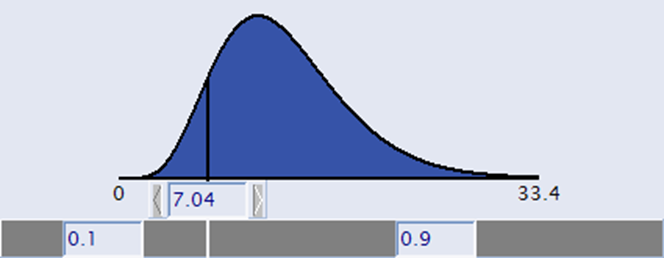
\includegraphics[scale=0.5]{ilustraciones/52.png} 
%ilustracion52%
\end{itemize}
\end{frame}

\section{Distribución t-Student}


\begin{frame}
\textbf{Distribuci\'on t-Student}

La variable aleatoria X tiene la distribución t de Student si su función de densidad de probabilidad es:
$$ f(x)=\dfrac{\Gamma \left(\frac{\nu +1}{2} \right) \left(1+\frac{x^2}{\nu}\right)^\frac{\nu +1}{2}}{\Gamma \left(\frac{\nu }{2}\right)\sqrt{\nu \pi}}$$
Donde $\nu$ es un n\'umero natural y se conoce con el nombre de \textit{grados de libertad}. 
\end{frame}

\begin{frame}{Distribuci\'on t-Student}

$$E(X)=\left\{\begin{matrix}
 0 & \nu\ge 2\\ 
& \\
\mbox{no existe} & \nu =1 
\end{matrix}\right.$$
$$Var(X)=\left\{\begin{matrix}
 \frac{\nu}{\nu -2} & \nu\ge 3\\ 
& \\
\mbox{no existe} & \nu <3 
\end{matrix}\right.$$

\end{frame}

\begin{frame}{Distribuci\'on t-Student}
\begin{center}
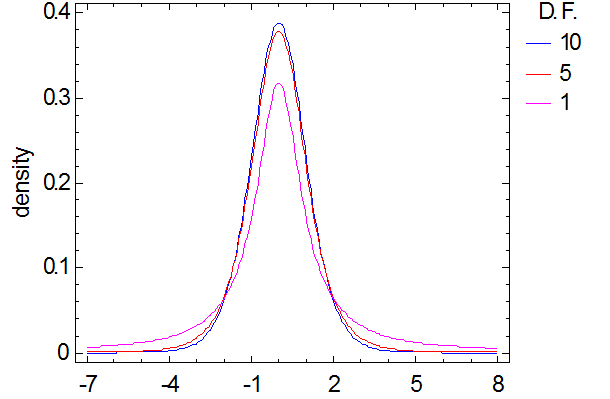
\includegraphics[scale=0.6]{ilustraciones/55.png} 
%ilustracion55%
\end{center}
\end{frame}

\begin{frame}{Distribuci\'on t-Student}
\begin{center}
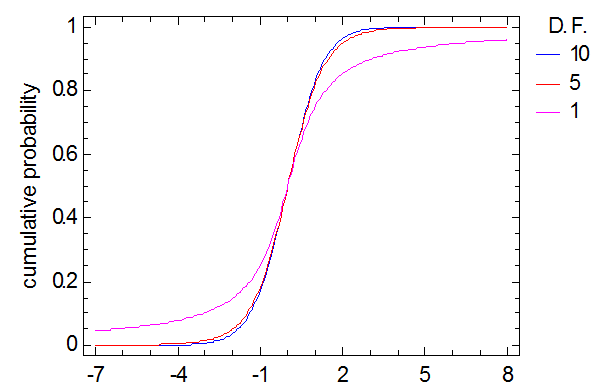
\includegraphics[scale=0.6]{ilustraciones/56.png} 
%ilustracion56%
\end{center}
\end{frame}

\begin{frame}{Utilizaci\'on}
\begin{itemize}
\item Debido al uso que le daremos, lo que nos interesa calcular de la distribuci\'on t de Student son sus Cuantiles. Es decir, los valores $x$ tales que $P(X\le x)$ es igual a un cierto $\alpha$.

\item Sea $X\sim { t }_{ (\nu ) },{ t }_{ \alpha ,\nu  }$ es el valor $x$ tal que $P(X\le x) = \alpha$. Es decir, el valor tal que la probabilidad de que una variable t de Student con n grados de libertad resulte menor que ese valor sea $\alpha$. Dicho de otra forma, el valor que tiene un área a a la izquierda, bajo la curva de una t de Student con $\nu$ grados de libertad.

\item Dichos cuantiles se encuentran en la tabla 2.
\end{itemize}
\end{frame}

\begin{frame}{Ejemplo de t de Student}

Sea $X \sim t_{(13)}$
\begin{itemize}
\item Se lee `'X es una variable t de Student con 13 grados de libertad''.

\item El valor ${ t }_{ 0.9,13 }$:Es el cuantil de la $t$ de Student para $\alpha = 0.9$ con $13$ grados de libertad.

\item Es decir:es el valor tal que hay probabilidad $0.9$ de que una variable $t$ de Student con $13$ grados de libertad resulte menor a \'el.

\item Es decir:es el valor tal que hay un \'area de $0.9$ a su izquierda, bajo la curva de la funci\'on de densidad de una variable t de Student con $\nu=13$.

\item Buscando en la tabla, vemos que vale: $1.35$
\end{itemize}
\end{frame}

\begin{frame}{Ejemplo de t de Student}
Sea $X:t_{(13)}$
\begin{itemize}
\item Se lee "X es una variable $t$ de Student con 13 grados de libertad".
\item El valor ${ t }_{ 0.9,13 }$:Es el cuantil de la $t$ de Student para $\alpha=0.9$ con 13 grados de libertad.

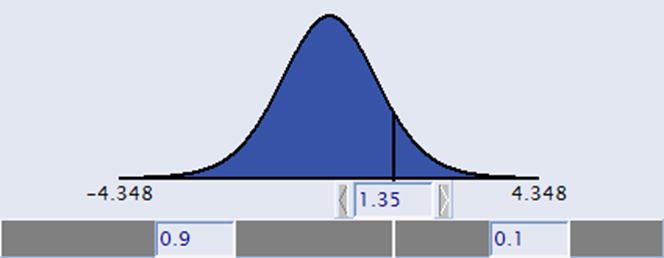
\includegraphics[scale=0.5]{ilustraciones/57.png} 
%ilustracion57%
\item Buscando en la tabla, vemos que vale:1.35
\end{itemize}
\end{frame}


\section{Distribución F de Fisher}


\begin{frame}{Distribuci\'on F}

La variable aleatoria $X$ tiene la distribución $F$ si su funci\'on de densidad de probabilidad es:
$$f(x)=\frac{\Gamma \left(\frac{n+m}{2} \right) }{\Gamma \left(\frac{n}{2}\right)\Gamma \left(\frac{m}{2}\right)} \left(\frac{m}{n}\right) ^\frac{m}{2} x^\frac{m-2}{2} \left( 1 + \frac{m}{n} x \right) ^{-\frac{n+m}{2}}$$

Donde $n$ y $m$ son n\'umeros naturales y se conocen como los "grados de libertad"

\end{frame}

\begin{frame}{Distribuci\'on F}
$$E(X)=\frac{n}{n-2}$$
$$Var(X)=\frac{2n^2 (n+n-2)}{m (n-2)^2 (n-4)}$$

\end{frame}

\begin{frame}{Distribuci\'on F}

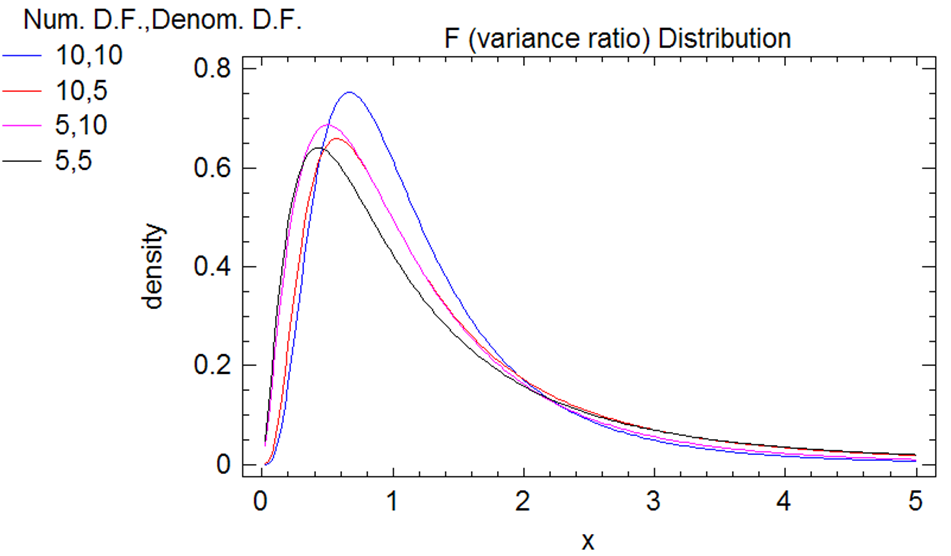
\includegraphics[scale=0.5]{ilustraciones/60.png} 
%ilustracion60%
\end{frame}


\begin{frame}{Distribuci\'on F}

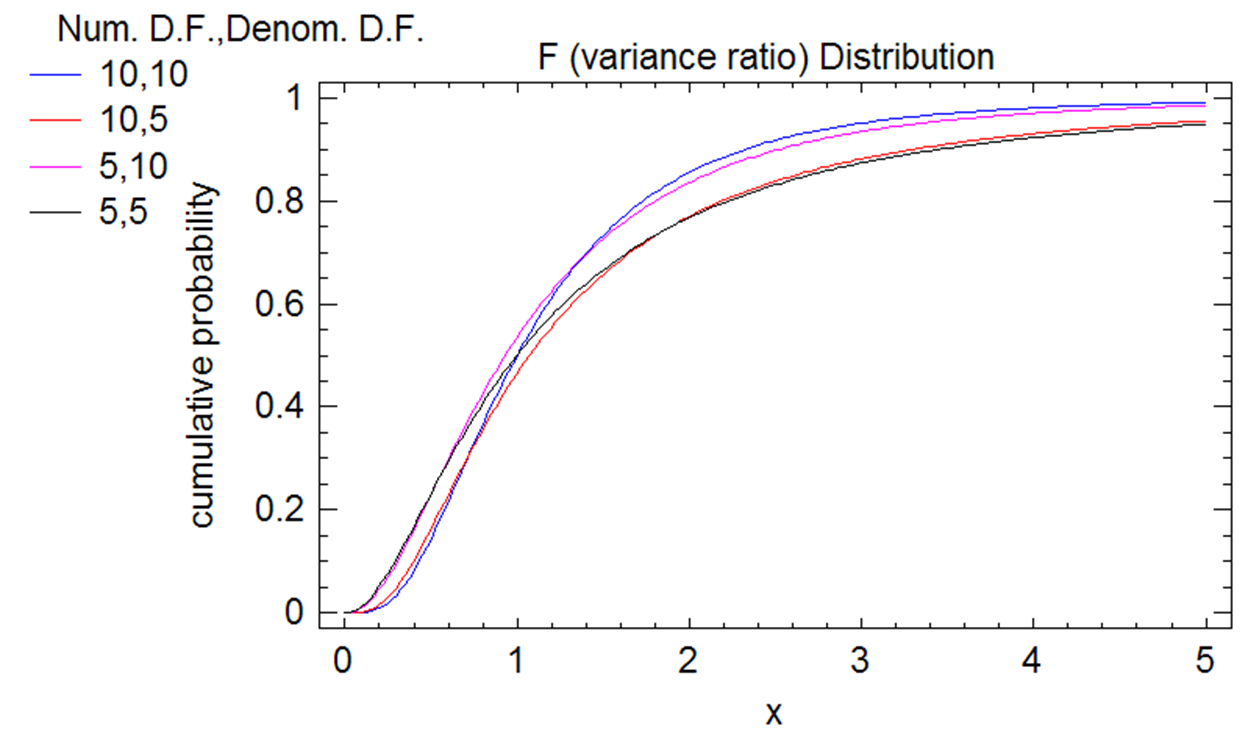
\includegraphics[scale=0.5]{ilustraciones/61.png} 
%ilustracion60%
\end{frame}


\begin{frame}{Utilizaci\'on}
\begin{itemize}
\item Debido al uso que le daremos, lo que nos interesa calcular de la distribución $F$ son sus Cuantiles. Es decir, los valores x tales que $P(X  \le x)$ es igual a un cierto $\alpha$.

\item Sea $X\sim { F }_{ (m,n) },{ f }_{ \alpha ,m,n }$ es el valor x tal que $P(X\le x)=\alpha$.Es decir, el valor tal que la probabilidad de que una variable F con m, n grados de libertad resulte menor que ese valor sea a.Dicho de otra forma, el valor que tiene un \'area a a la izquierda, bajo la curva de una F con m,n grados de libertad.

\item Dichos cuantiles se encuentran en la tabla 4.
\end{itemize}
\end{frame}

\begin{frame}{Nota}
\begin{itemize}
\item Muchos autores trabajan con el cuantil de la F a derecha en vez de a izquierda.
 
\item Recomendaci\'n: al consultar una tabla verificar previamente si los cuantiles son a la izquierda o a la derecha. 

\item Una propiedad importante a tener en cuenta es:
$$ F_{\alpha , m , n} = \frac{1}{F_{1-\alpha ,n , m}}$$

\item Es decir, el cuantil de \'area a de una F con par\'ametros m y n, es uno sobre el cuantil de \'area 1-a de una F con par\'ametros n y m (es decir, intercambiados).
\end{itemize}
\end{frame}

\begin{frame}{Ejemplo de F}

Sea $X:{ F }_{ 5,10 }$
\begin{itemize}
\item Se lee `'X es una variable F con $m=5$ y $n=10$ grados de libertad''.

\item El valor ${ F }_{ 0.95;5,10}$:Es el cuantil de la F para $\alpha=0.95$ con $m=5$ y $n=10$ grados de libertad.

\item Es decir: es el valor tal que hay probabilidad 0.95 de que una variable F con $m=5$ y $n=10$ grados de libertad resulte menor a \'el.

\item Es decir: es el valor tal que hay un \'area de 0.95 a su izquierda, bajo la curva de la funci\'on de densidad de una variable F con $m=5$ y $n=10$.

\item Buscando en la tabla, vemos que vale:3.33
\end{itemize}
\end{frame}

\begin{frame}{Ejemplo de F}

Sea $X:{ F }_{ 5,10 }$
\begin{itemize}
\item Se lee "X es una variable F con m=5 y n=10 grados de libertad".
\item El valor ${ F }_{ 0.95;5,10}$:Es el cuantil de la F para $\alpha=0.95$ con $m=5$ y $n=10$ grados de libertad.
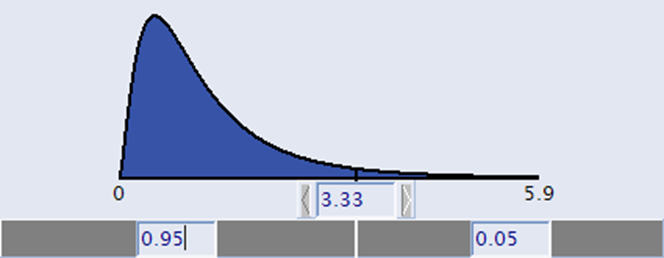
\includegraphics[scale=.5]{ilustraciones/63.png} 
%ilustracion63%
\item  Buscando en la tabla, vemos que vale:3.33
\end{itemize}
\end{frame}


\section{* Distribución Exponencial}



\begin{frame}{Distribuciónn Exponencial}

Se dice que X tiene una distribución exponencial si tiene las siguiente forma:

$$F(x)=1-e^{-\lambda x}.  \hspace{25pt}  x>0$$

$$f(x)=\frac{dF(x)}{dx}=\lambda e^{-\lambda x} , \hspace{20pt}  x>0$$

$$E(X) = \frac{1}{\lambda} \hspace{20pt} Var(X)=\frac{1}{\lambda ^2}$$


\end{frame}


\begin{frame}{Distribuci\'on Exponencial}
\begin{center}
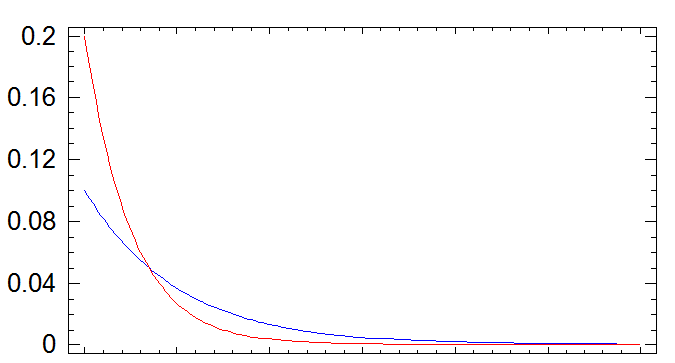
\includegraphics[scale=0.5]{ilustraciones/65.png} 
%ilustracion65%
\end{center}
\end{frame}

\begin{frame}{Distribuci\'on Exponencial}
\begin{center}
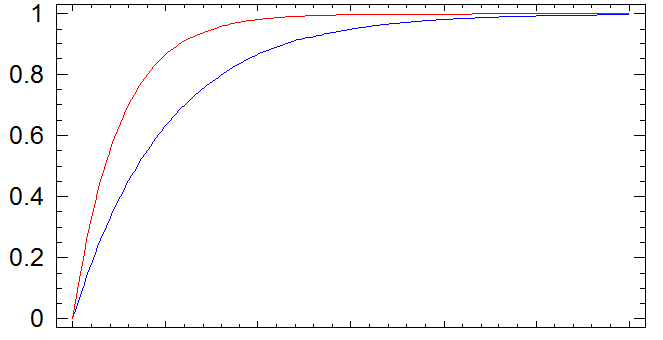
\includegraphics[scale=0.5]{ilustraciones/66.png} 
%ilustracion66%
\end{center}
\end{frame}

\begin{frame}{Ejemplo de v.a. exponencial}

Suponga que el tiempo de respuesta X en cierta Terminal de computadora en línea tiene una distribución exponencial con tiempo esperado de respuesta igual a 5 s.

\bigskip
Entonces $E(X)=\frac { 1 }{ \lambda  } =5$ por lo cual $\lambda =0.2$.
\begin{itemize}
\item Determine la  probabilidad de que el tiempo de respuesta sea a lo sumo 10.
\item Determine la probabilidad de que el tiempo de respuesta este entre 5 y 10.
\end{itemize}

\end{frame}

\begin{frame}{Ejemplo de v.a. exponencial}
\begin{itemize}
\item Determine la  probabilidad de que el tiempo de respuesta sea a lo sumo 10.

$P(X\le 10)=F(10;0.2)=1-e^{- (0.2)(10)} =1-e^{- 2}= 1 - .135 =.865$


\item Determine la probabilidad de que el tiempo de respuesta este entre 5 y 10.

$P(5 \le X \le 10)= F(10; 0.2) - F(5 ; 0.2) $

$P(5 \le X \le 10)= (1-e^{- (0.2)(10)})-(1-e^{- (0.2)(5)}) =0.233$
\end{itemize}
\end{frame}





\begin{frame}{Aplicaciones de la distribuci\'on exponencial}

La distribuci\'on exponencial se utiliza con frecuencia como modelo para la distribuci\'on de tiempos entre la presentaci\'on de eventos sucesivos, como es el caso de clientes que llegan a un taller de servicio o llamadas que entran en un conmutador. 
\end{frame}


\begin{frame}{Aplicaciones de la distribuci\'on exponencial}
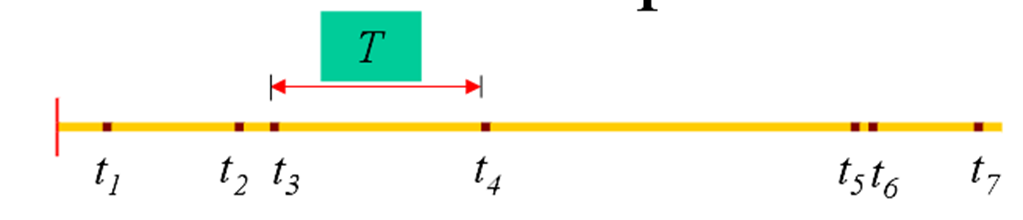
\includegraphics[scale=0.5]{ilustraciones/69.png} 
%ilustracion69% 

Ejemplo: Fabricación continua de conductor de cobre.

\bigskip
$\lambda=$Número medio de defectos cada 100 m

\bigskip
$T=$Distancia entre dos defectos
\end{frame}

\begin{frame}{Propiedades (Exponencial)}

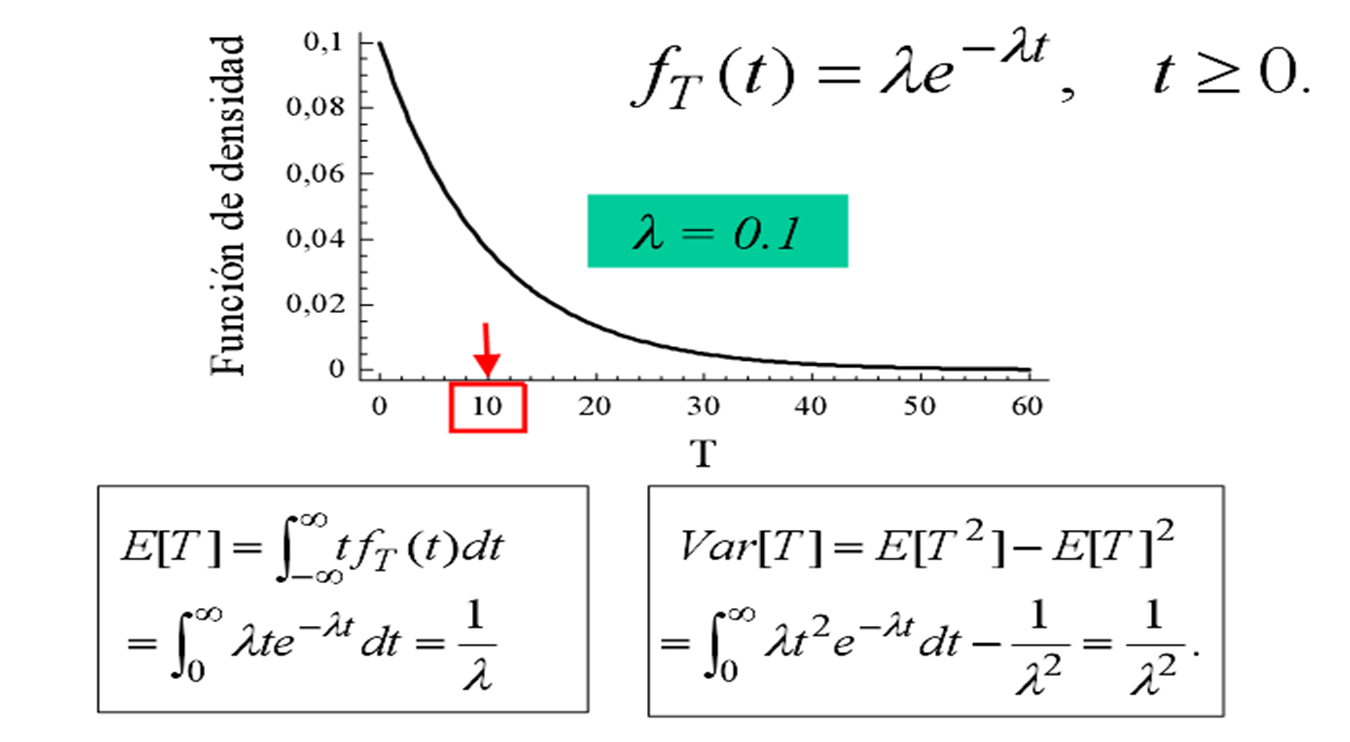
\includegraphics[scale=0.5]{ilustraciones/70.png} 
%ilustracion70%
\end{frame}

\section{* Distribución Weibull}



\begin{frame}{*** Distribuci\'on Weibull}
Se dice que X tiene una distribuci\'on Weibull si tiene la siguiente forma:
    $$F(x)=1-exp {\left[- \left( \frac{x}{\alpha}\right)^\beta \right]} \mbox{, }x>0$$
    $$ f(x)=\left( \frac{\beta}{\alpha} \right) \left( \frac{x}{\alpha} \right) ^{\beta -1} exp {\left[- \left( \frac{x}{\alpha}\right)^\beta \right]} \mbox{, } x>0$$
    

$$E(X)=\alpha \Gamma \left( \beta ^ {-1} +1 \right)$$
$$Var(X)=\alpha^2 \left[\Gamma \left(2\beta^{-1}+1\right) - \left[ \Gamma \left( \beta^{-1}+1\right)\right]^2 \right]$$

\end{frame}

\begin{frame}
\newpage
\begin{Large}
\begin{flushleft}
\textbf{*** Distribuci\'on Weibull}
\end{flushleft}
\end{Large}
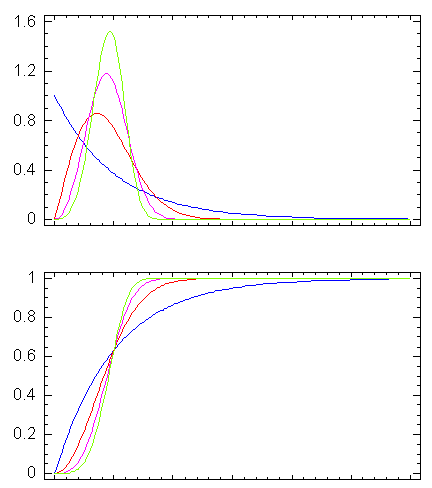
\includegraphics[scale=0.5]{ilustraciones/73.png} 
%ilustracion73%
\end{frame}


\section{Resumen}
\begin{frame}{Principales distribuciones de probabilidad contínuas}

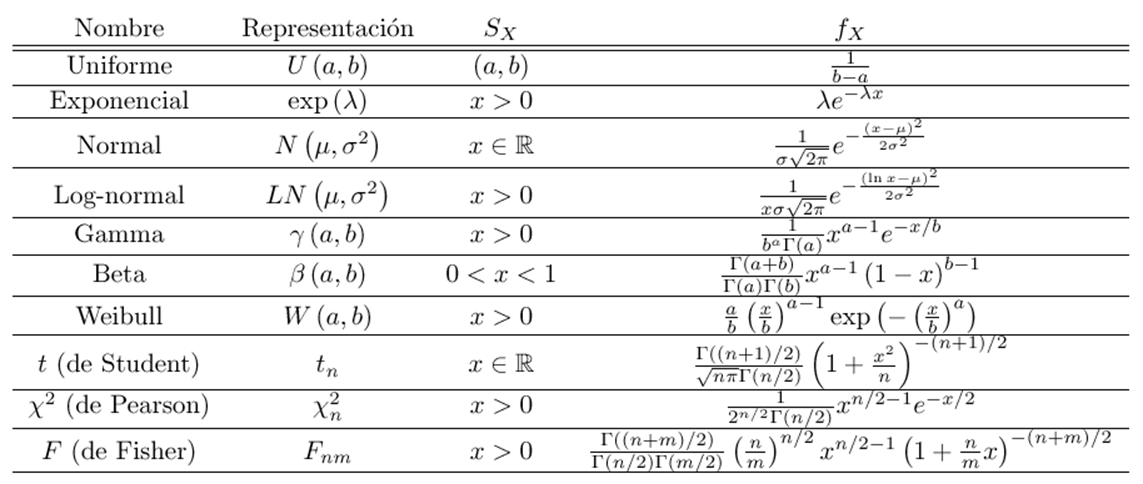
\includegraphics[scale=0.55]{ilustraciones/77.png} 
%ilustracion77%
\end{frame}


\begin{frame}{Principales distribuciones de probabilidad contínuas}

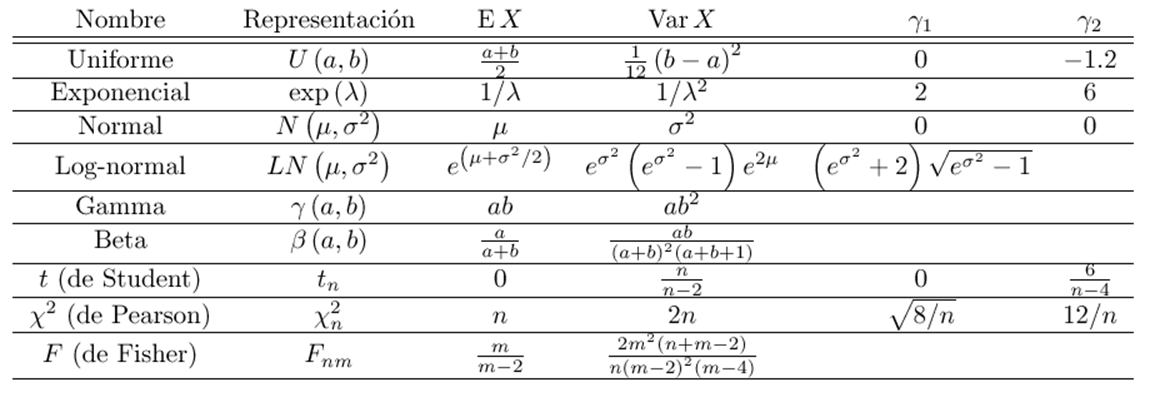
\includegraphics[scale=0.55]{ilustraciones/78.png} 
%ilustracion78%
\end{frame}


\section{Distribuciones contínuas conjuntas}
\subsection{Función de probabilidad conjunta}


\begin{frame}{Función de densidad conjunta}
Una función bivariada con valores $f(x,y)$, definida sobre el plano $xy$, se llama {\bf función de densidad de probabilidad conjunta} de las variables aleatorias $X$ y $Y$ si y sólo si

$$P[(X,Y) \in A]= \int_A \int {f(x,y) \, dx    \, dy }.$$
para cualquier región $A$ en el plano $xy$.

\bigskip
se puede mostrar que satisfacen las siguientes condiciones
\begin{enumerate}
\item $f(x,y) \ge 0 \quad \mbox{ para } -\infty < x < \infty , -\infty < y < \infty ;$
\item $  \int_{-\infty}^{\infty} \int_{-\infty}^{\infty} {f(x,y) \, dx    \, dy } =1 $
\end{enumerate}
\end{frame}


\begin{frame}{Ejemplo}
Dada la función de densidad de probabilidad conjunta
$$ f(x,y) =\left\{ \begin {matrix} 
\frac{3}{5}x(y+x) & \mbox{para } 0<x<1,0<y<2 \\ 
0 & \mbox{en cualquier otra parte}
\end{matrix} \right . $$
de dos variables aleatorias $X$ y $Y$, encuentre $P[(X,Y) \in A]$, donde $A$ es la región $\{(x,y) \mid 0<x<\frac{1}{2}, 1<y<2\}$.
\end{frame}


\begin{frame}{Ejemplo}

\begin{eqnarray*}
P[(X,Y) \in A] &=&P \bigg( 0 <X<\frac{1}{2},1<Y<2 \bigg)  \\
&=&   \int_{1}^{2} {\int_{0}^{\frac{1}{2}} { \frac{3}{5}x(y+x) \, dx   } \, dy } \\
&=&  \int_{1}^{2} { \frac{3x^2 y}{10}+\frac{3x^3}{15} \bigg|_{0}^{\frac{1}{2}}    dy } \\
&=&  \int_{1}^{2} { \bigg(  \frac{3y}{40}+\frac{1}{40} \bigg)   dy } \\
&=&  \frac{3y^2}{80}+\frac{y}{40} \bigg|_1^2 \\
&=& \frac{11}{80}
\end{eqnarray*}
\end{frame}

\begin{frame}{Función de distribución conjunta}
Si  $X$ y $Y$ son variables aleatorias contínuas, la función dada por 

$$F(x,y)=P(X\le x,Y \le y)= \int_{-\infty}^{y} \int_{- \infty}^{x} {f(s,t) \, ds    \, dt }$$ para $ -\infty < x < \infty , -\infty < y < \infty $

donde $f(s,t)$ es el valor de la densidad de probabilidad conjunta de $X$ y $Y$ en $(s,t)$, se llama la {\bf función de distribución conjunta } de $X$ y $Y$.
\end{frame}


\begin{frame}{Ejemplo}
Dada la función de densidad de probabilidad conjunta
$$ f(x,y) =\left\{ \begin {matrix} 
(y+x) & \mbox{para } 0<x<1,0<y<1 \\ 
0 & \mbox{en cualquier otra parte}
\end{matrix} \right . $$
encuentre la función de distribución conjunta de estas dos variables aleatorias.

{\bf Solución}

de dos variables aleatorias $X$ y $Y$, encuentre $P[(X,Y) \in A]$, donde $A$ es la región $\{(x,y) \mid 0<x<\frac{1}{2}, 1<y<2\}$.
\end{frame}

\begin{frame}{Ejemplo}
Si $x<0$ o $u<0$, se sigue que $F(x,y)=0$. Para $0<x<1$ y $0<y<1$ (Región I) obtenemos 
$$ F(x,y)=\int_{0}^{y} \int_{0}^{x} {(s+t) \, ds    \, dt } = \frac{1}{2}xy(x+y) $$ para $x>1$ y $0<y<1$ (Región II), obtenemos  
$$ F(x,y)=\int_{0}^{y} \int_{0}^{1} {(s+t) \, ds    \, dt } = \frac{1}{2}y(y+1) $$ para 
$0<x<1$ y $y>1$ (Región III), obtenemos  
$$ F(x,y)=\int_{0}^{1} \int_{0}^{x} {(s+t) \, ds    \, dt } = \frac{1}{2}x(x+1) $$ y para
$x>1$ y $y>1$ (Región IV), obtenemos  
$$ F(x,y)=\int_{0}^{1} \int_{0}^{1} {(s+t) \, ds    \, dt } = 1. $$

\end{frame}
\begin{frame}{Ejemplo}
$$F(x,y)=\left\{ \begin{matrix}
 0 & x<0 \mbox{ o } y<0 \\ \\
 \dfrac{1}{2}xy(x+y)  & 0<x<1 \mbox{ y } 0<y<1 \\ \\
 \dfrac{1}{2}y(y+1) & x>1 \mbox{ y } 0<y<1 \\ \\
  \dfrac{1}{2}x(x+1)  &  0<x<1\mbox{ y } y>1  \\ \\
  1 &  x>1 \mbox{ y } y>1
  \end{matrix} \right .$$

\end{frame}

\begin{frame}{Función de distribución conjunta}
Análogamente  a la relación $$f(x)=\frac{d F(x)}{dx}$$  la diferenciación parcial de $F$ nos lleva a $$f(x,y)=\frac{ \delta^2}{\delta x \delta y} F(x,y)$$ en todas partes donde exista estas derivadas parciales.

\end{frame}



\begin{frame}{Ejemplo}
Encuentre la densidad de probabilidad conjunta de las dos variables aleatorias $X$ y $Y$  cuya función de distribución conjunta está dada por $$F(x,y)= \left\{ \begin{matrix}
 (1-e^{-x})(1-e^{-y}) & \mbox{para } x>0 \mbox{ y } y>0 \\
0 & \mbox{en cualquier otra parte}
\end{matrix} \right . $$
Además use la función de densidad conjunta para determinar $$P(1<X<3,1<Y<2).$$
\end{frame}



\begin{frame}{Ejemplo}
{\bf Solución}
Puesto que la diferenciación parcial nos da $$f(x,y)=\frac{ \delta^2}{\delta x \delta y} F(x,y)=e^{-(x+y)}$$ para $x>0$ y $y>0$ y $0$ en cualquier otra parte, encontramos que la densidad de probabilidad conjunta de $X$ y $Y$ está dada por 
$$ f(x,y) =\left\{ \begin {matrix} 
e^{-(x+y)} & \mbox{para } x>0, y>0 \\ 
0 & \mbox{en cualquier otra parte}
\end{matrix} \right . $$


\end{frame}


\begin{frame}{Ejemplo}
Así la integración nos da
\begin{eqnarray*}
P(1<X<3,1<Y<2) &=& \int_{1}^{2} {\int_{1}^{3} {e^{-(x+y)}} \, dx    \, dy }  \\
&=& (e^{-1} - e^{-3})(e^{-1}-e^{-3}) \\
&=& e^{-2} - e^{-3}-e^{-4}+e^{-5} \\
&=& 0.074
\end{eqnarray*}

\end{frame}


\begin{frame}{Ejemplo}
\begin{center}
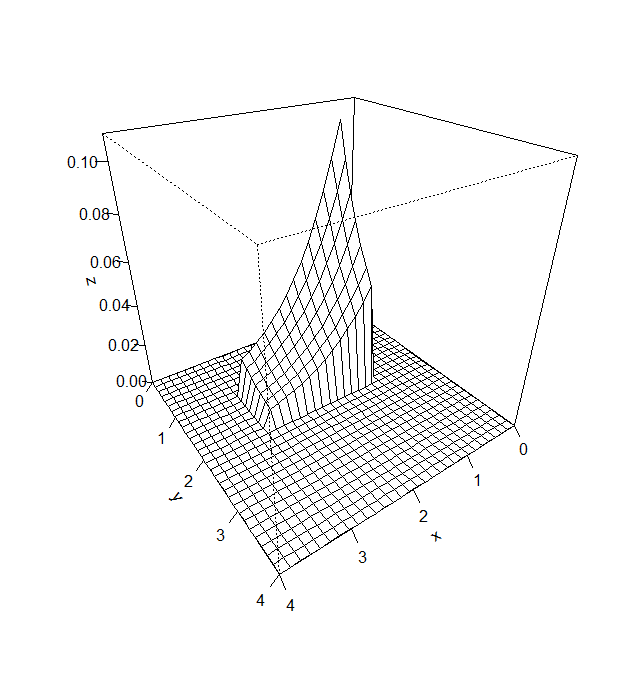
\includegraphics[scale=.45]{ilustraciones/exp(-(x+y)).png} 
\end{center}

\end{frame}



\subsection{Función de probabilidad marginal}
\begin{frame}{Función de probabilidad marginal}
Si $X$ y $Y$ son variables aleatorias continuas y $f(x,y)$ es el valor de la densidad de probabilidad conjunta en $(x,y)$ la función dad por 
$$g(x)=\int_{-\infty}^{\infty}{f(x,y)\; dy} \mbox{ para } -\infty <x<\infty$$
se llama la {\bf densidad marginal} de $X$. Correspondientemente, la función dada por 
$$h(y)=\int_{-\infty}^{\infty}{f(x,y)\; dx} \mbox{ para } -\infty <y<\infty$$
se llama la {\bf densidad marginal} de $Y$. 
\end{frame}


\begin{frame}{Ejemplo}
Dada la densidad de probabilidad conjunta 
$$ f(x,y) =\left\{ \begin {matrix} 
\dfrac{2}{3}(x+2y) & \mbox{para } 0<x<1, 0<y<1 \\ 
0 & \mbox{en cualquier otra parte}
\end{matrix} \right . $$
encuentre las funciones de densidad marginal de $X$ y $Y$.


\end{frame}


\begin{frame}{Ejemplo}
{\bf solución}

Al efectuar las integraciones necesarias, obtenemos 
$$ g(x) =\int_{-\infty}^{\infty}{f(x,y)\; dy} =\int_{0}^{1}{\dfrac{2}{3}(x+2y)  \; dy}= \dfrac{2}{3}(x+1)$$  para $ -\infty <x<\infty $ y $g(x)=0$ en cualquier otra parte. De igual manera
$$h(y) =\int_{-\infty}^{\infty}{f(x,y)\; dx} =\int_{0}^{1}{\dfrac{2}{3}(x+2y)  \; dx}= \dfrac{1}{3}(1+4y)$$  para $ -\infty <y<\infty $ y $h(x)=0$  en cualquier otra parte.
\end{frame}



\subsection{Función de probabilidad condicional}
\begin{frame}{Función de probabilidad condicional}

Si $f(X,y)$ es el valor de la distribución de probabilidad conjunta de las variables aleatorias continuas $X$ y $Y$ en $(x,y)$, y $h(y)$ es el valor de la distribución marginal de $Y$ en $y$, la función dada por $$ f(x \mid y)=\frac{(x, y)}{h(y)} \hspace{20pt} h(y) \ne 0$$
para cada $x$ dentro del intervalo de $X$, se llama la {\bf distribución condicional} de $X$ dado $Y=y$. En forma correspondiente, si $g(x)$ es el valor de la distribución marginal de $X$ en $x$, la función dada por $$w(y \mid x)=\frac{(x, y)}{g(x)} \hspace{20pt} g(x) \ne 0$$
para cada $y$ dentro del intervalo de $Y$, se llama la {\bf distribución condicional} de $Y$ dado $X=x$.
\end{frame}


\begin{frame}{Ejemplo}

Dado
$$
f(x,y) =\left\{ \begin {matrix} 
\dfrac{2}{3}(x+2y) & \mbox{para } 0<x<1, 0<y<1 \\ 
0 & \mbox{en cualquier otra parte}
\end{matrix} \right . $$ 
Encuentre la densidad condicional de $X$ dado $Y=y$ y úsela para evaluar $P(X \le \frac{1}{2} \mid Y=\frac{1}{2}).$
\end{frame}


\begin{frame}{}

 {\bf Solución}
 \begin{eqnarray*}
f(x \mid y) &=& \frac{f(x,y)}{h(y)}  \\
&=&  \frac{ \frac{2}{3}(x+2y)}{ \frac{1}{3} (1+4y)}\\
&=& \frac{2x+4y}{1+4y}
\end{eqnarray*}
para $0<x<1$ y $f(x \mid y)=0$ en cualquier otra parte.
 Ahora
  \begin{eqnarray*}
f(x \mid \frac{1}{2} ) &=&  \frac{2x+4 \cdot \frac{1}{2}}{1+4 \cdot \frac{1}{2}} \\
&=& \frac{2x +2}{3}
\end{eqnarray*}
y podemos escribir
$$P(X \le \frac{1}{2} \mid Y=\frac{1}{2})= \int_0^{\frac{1}{2}}{\frac{2x+2}{3} \; dx}=\frac{5}{12}$$
\end{frame}


\subsection{Variables aleatorias independientes}
\begin{frame}{Variables aleatorias independientes}
Cuando trabajamos con dos o más variables aleatorias, generalmente es de gran importancia las preguntas de {\bf independencia}.  Siempre que los valores de la distribución condicional de $X$ dado $Y=y$ no depende de $y$, se sigue que $f(x \mid y)=g(x)$, y por tanto $$f(x,y)=f(x \mid y)h(y)=g(x)h(y)$$.

\end{frame}
\subsection{Ejemplo}
\begin{frame}{Ejemplo}
Dada la función de densidad de probabilidad conjunta 
$$
f(x,y) =\left\{ \begin {matrix} 
4xy & \mbox{para } 0<x<1, 0<y<1 \\ 
0 & \mbox{en cualquier otra parte}
\end{matrix} \right . $$ 
Al obtener las integraciones necesarias, obtenemos
  \begin{eqnarray*}
g(x) &=&   \int_{- \infty}^{\infty}{f(x,y) \; dy}=\int_{0}^{1}{4xy \; dy}\\ 
&=& 2xy^2 \big|_{y=0}^{y=1}=2x
\end{eqnarray*}
para $0<x<1$, y $g(x)=0$ en cualquier otra parte; también
  \begin{eqnarray*}
h(y) &=&   \int_{- \infty}^{\infty}{f(x,y) \; dx}=\int_{0}^{1}{4xy \; dx}\\ 
&=& 2x^2y \big|_{x=0}^{y=1}=2y
\end{eqnarray*}
para $0<y<1$, y $h(y)=0$ en cualquier otra parte.
\end{frame}


\begin{frame}{Ejemplo}
Entonces, al sustituir en la fórmula para la densidad condicional, obtenemos 
$$f(x \mid y)=\frac{f(x,y)}{h(y)} = \frac{4xy}{2y}=2x$$ Como vemos $f(x \mid y)$ no depende del valor de $Y=y$ y no depende de $y$, como puede ver $f(x \mid y)=g(x)$ . Como puede observar 
$$ f(x,y)=4xy = (2x)(2y)=g(x)h(y)$$
es decir $X$ y $Y$ son independientes.
\end{frame}


\begin{frame}{Propiedades}
A su vez, conociendo la función de densidad marginal y condicional, se puede producir la distribución conjunta
\begin{eqnarray*}
f(x,y)&=&f(x\mid y)\cdot h(y) \\
f(x,y)&=&f(y\mid x)\cdot g(x) 
\end{eqnarray*}
Las variables aleatorias $X$ y $Y$ serán independientes estadísticamente si las probabilidades condicionales son identicas a las marginales
\begin{eqnarray*}
f(x\mid y) &=&g(x) \\
f(y\mid x)&=& h(y) 
\end{eqnarray*}

\end{frame}




\end{document}

